% !TeX root = ..\main.tex

\chapter{Realizace}
V této kapitole je popsaná metoda měření, charakterizace pneumatického systému, analýza analogově digitálních převodníků a ukázka naměřených pulzací systémem CarDi.

\section{Deska plošného spoje}
Na desce plošného spoje (DPS) sídlí všechny elektrické komponenty pro řízení systému, sběr a vyhodnocení dat.
\begin{figure}[H]
    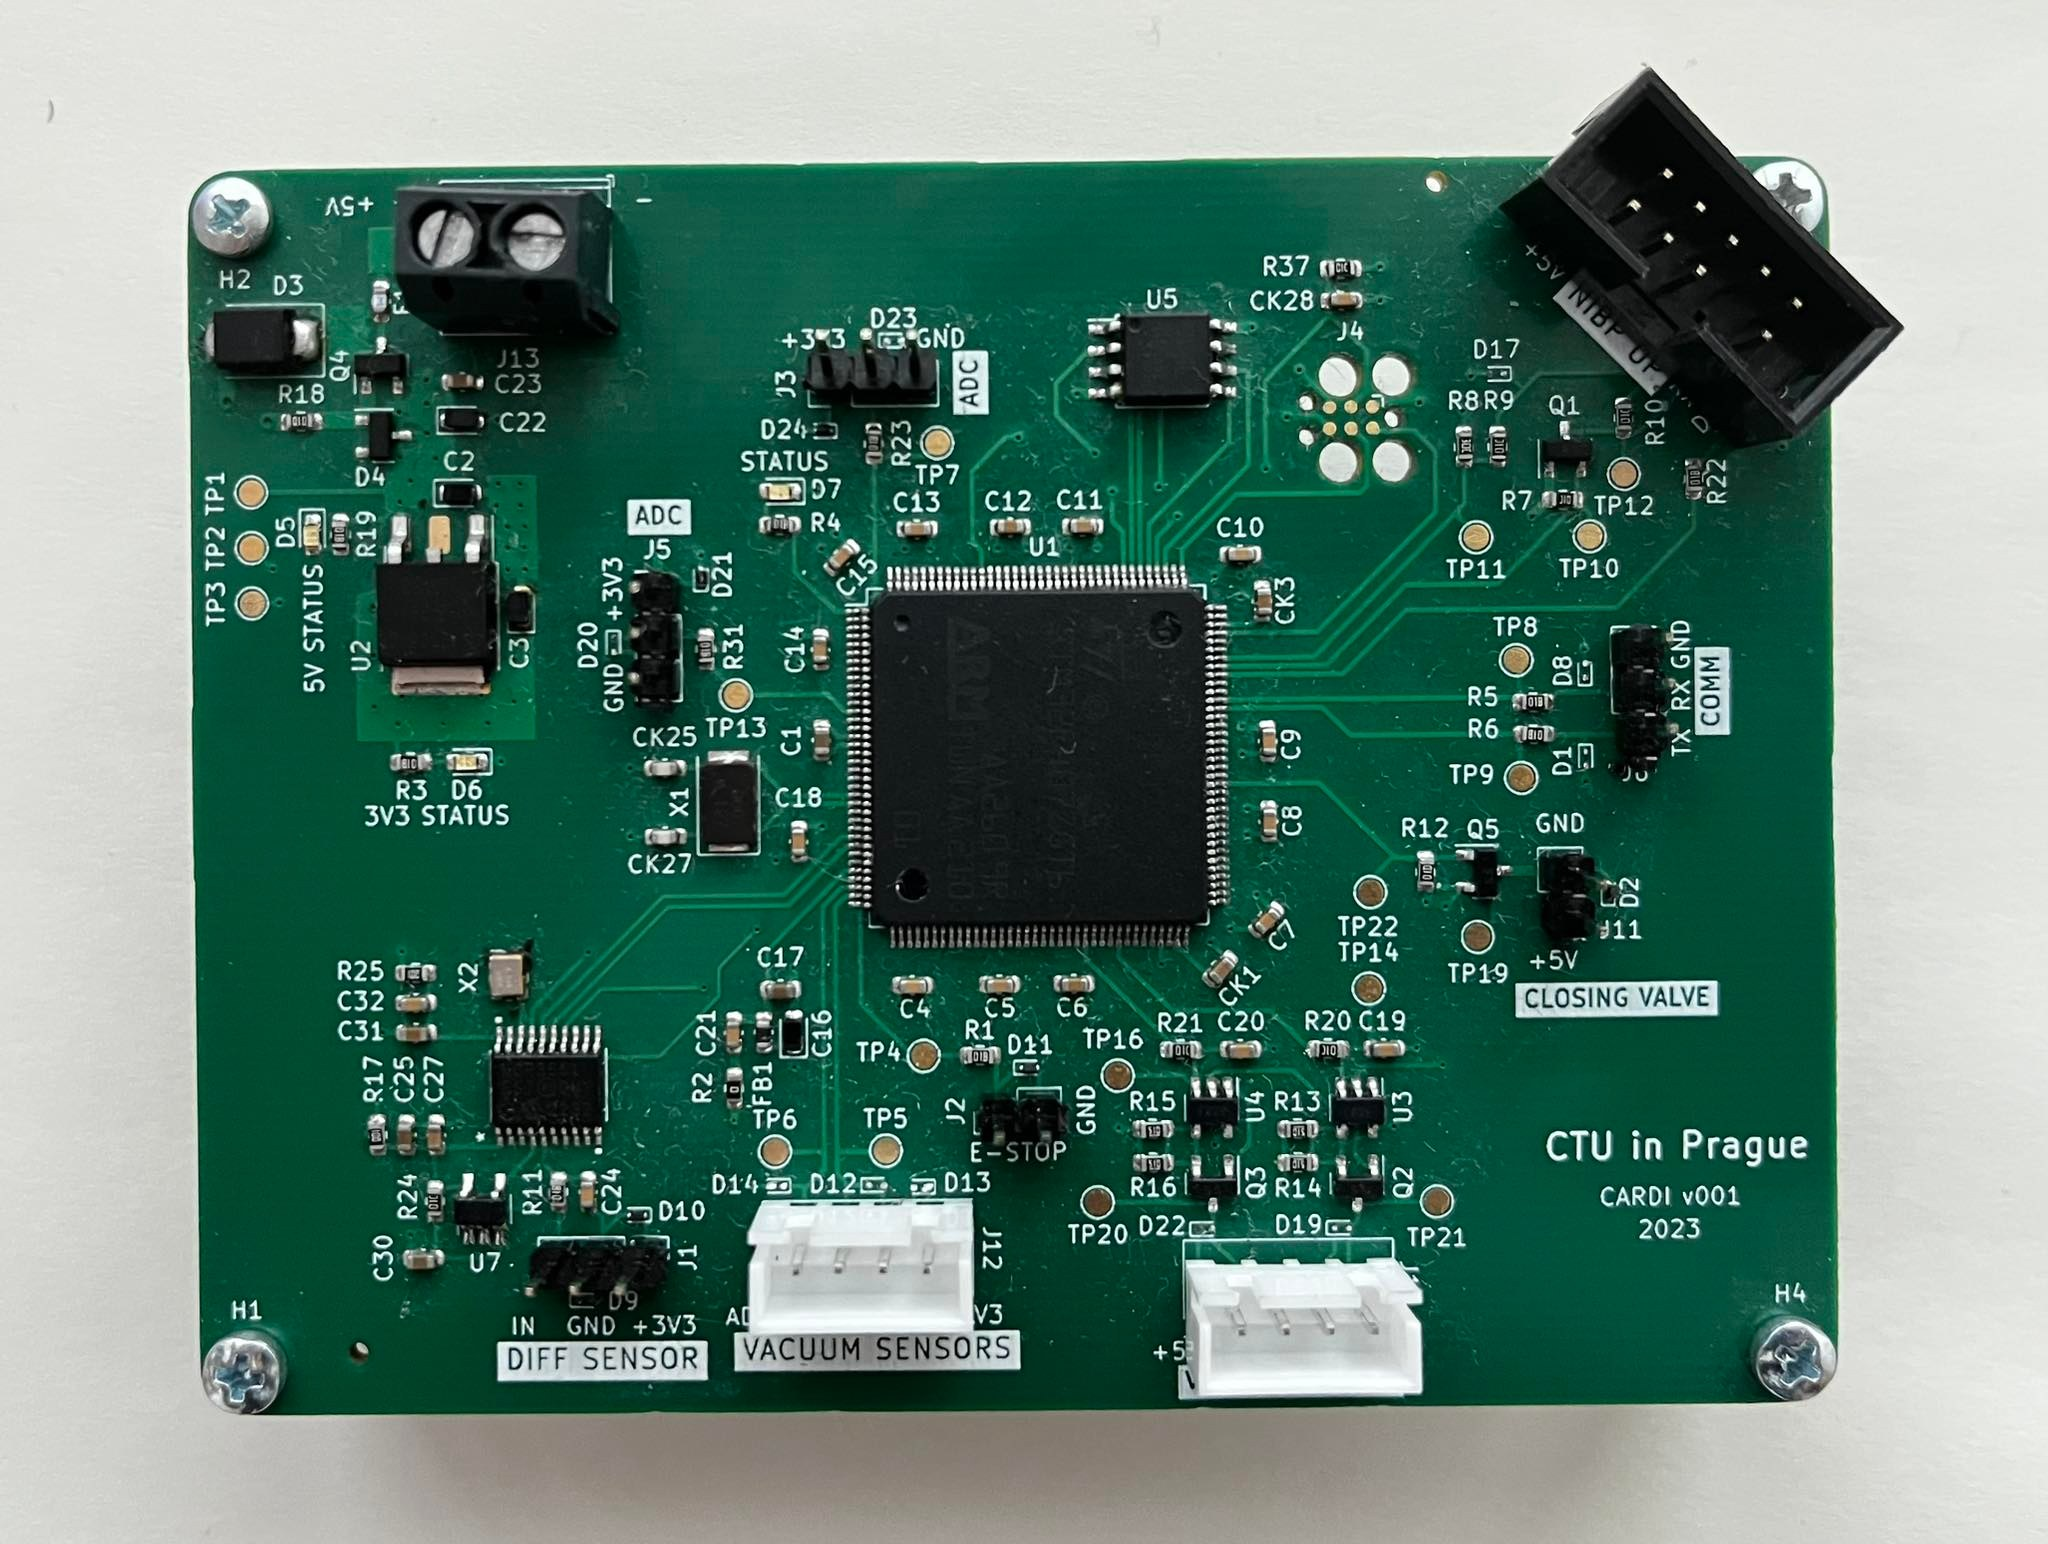
\includegraphics[width=1\linewidth]{pictures/pcb_full.jpg}
    \caption{Realizovaná deska plošného spoje.}
    \label{fig:pcb_full}
\end{figure}

DPS je čtyřvrstvá deska o výšce 1.6 mm se základním materiálem FR-4 a povrchovou úpravou ENIG(Electroless nickel immersion gold). DPS obsahuje dvě signálové a dvě silové vrstvy, kde první(horní) vrstva je signálová a nachází se na ní veškeré elektronické komponenty, druhá je společná zem, třetí je napájecí 3.3 V a poslední spodní vrstva je také signálová.
\par
DPS a schéma je navržena v otevřeném freeware KiCad EDA a je vyrobena a z části osazena firmou JLCPCB.
\begin{figure}[H]
    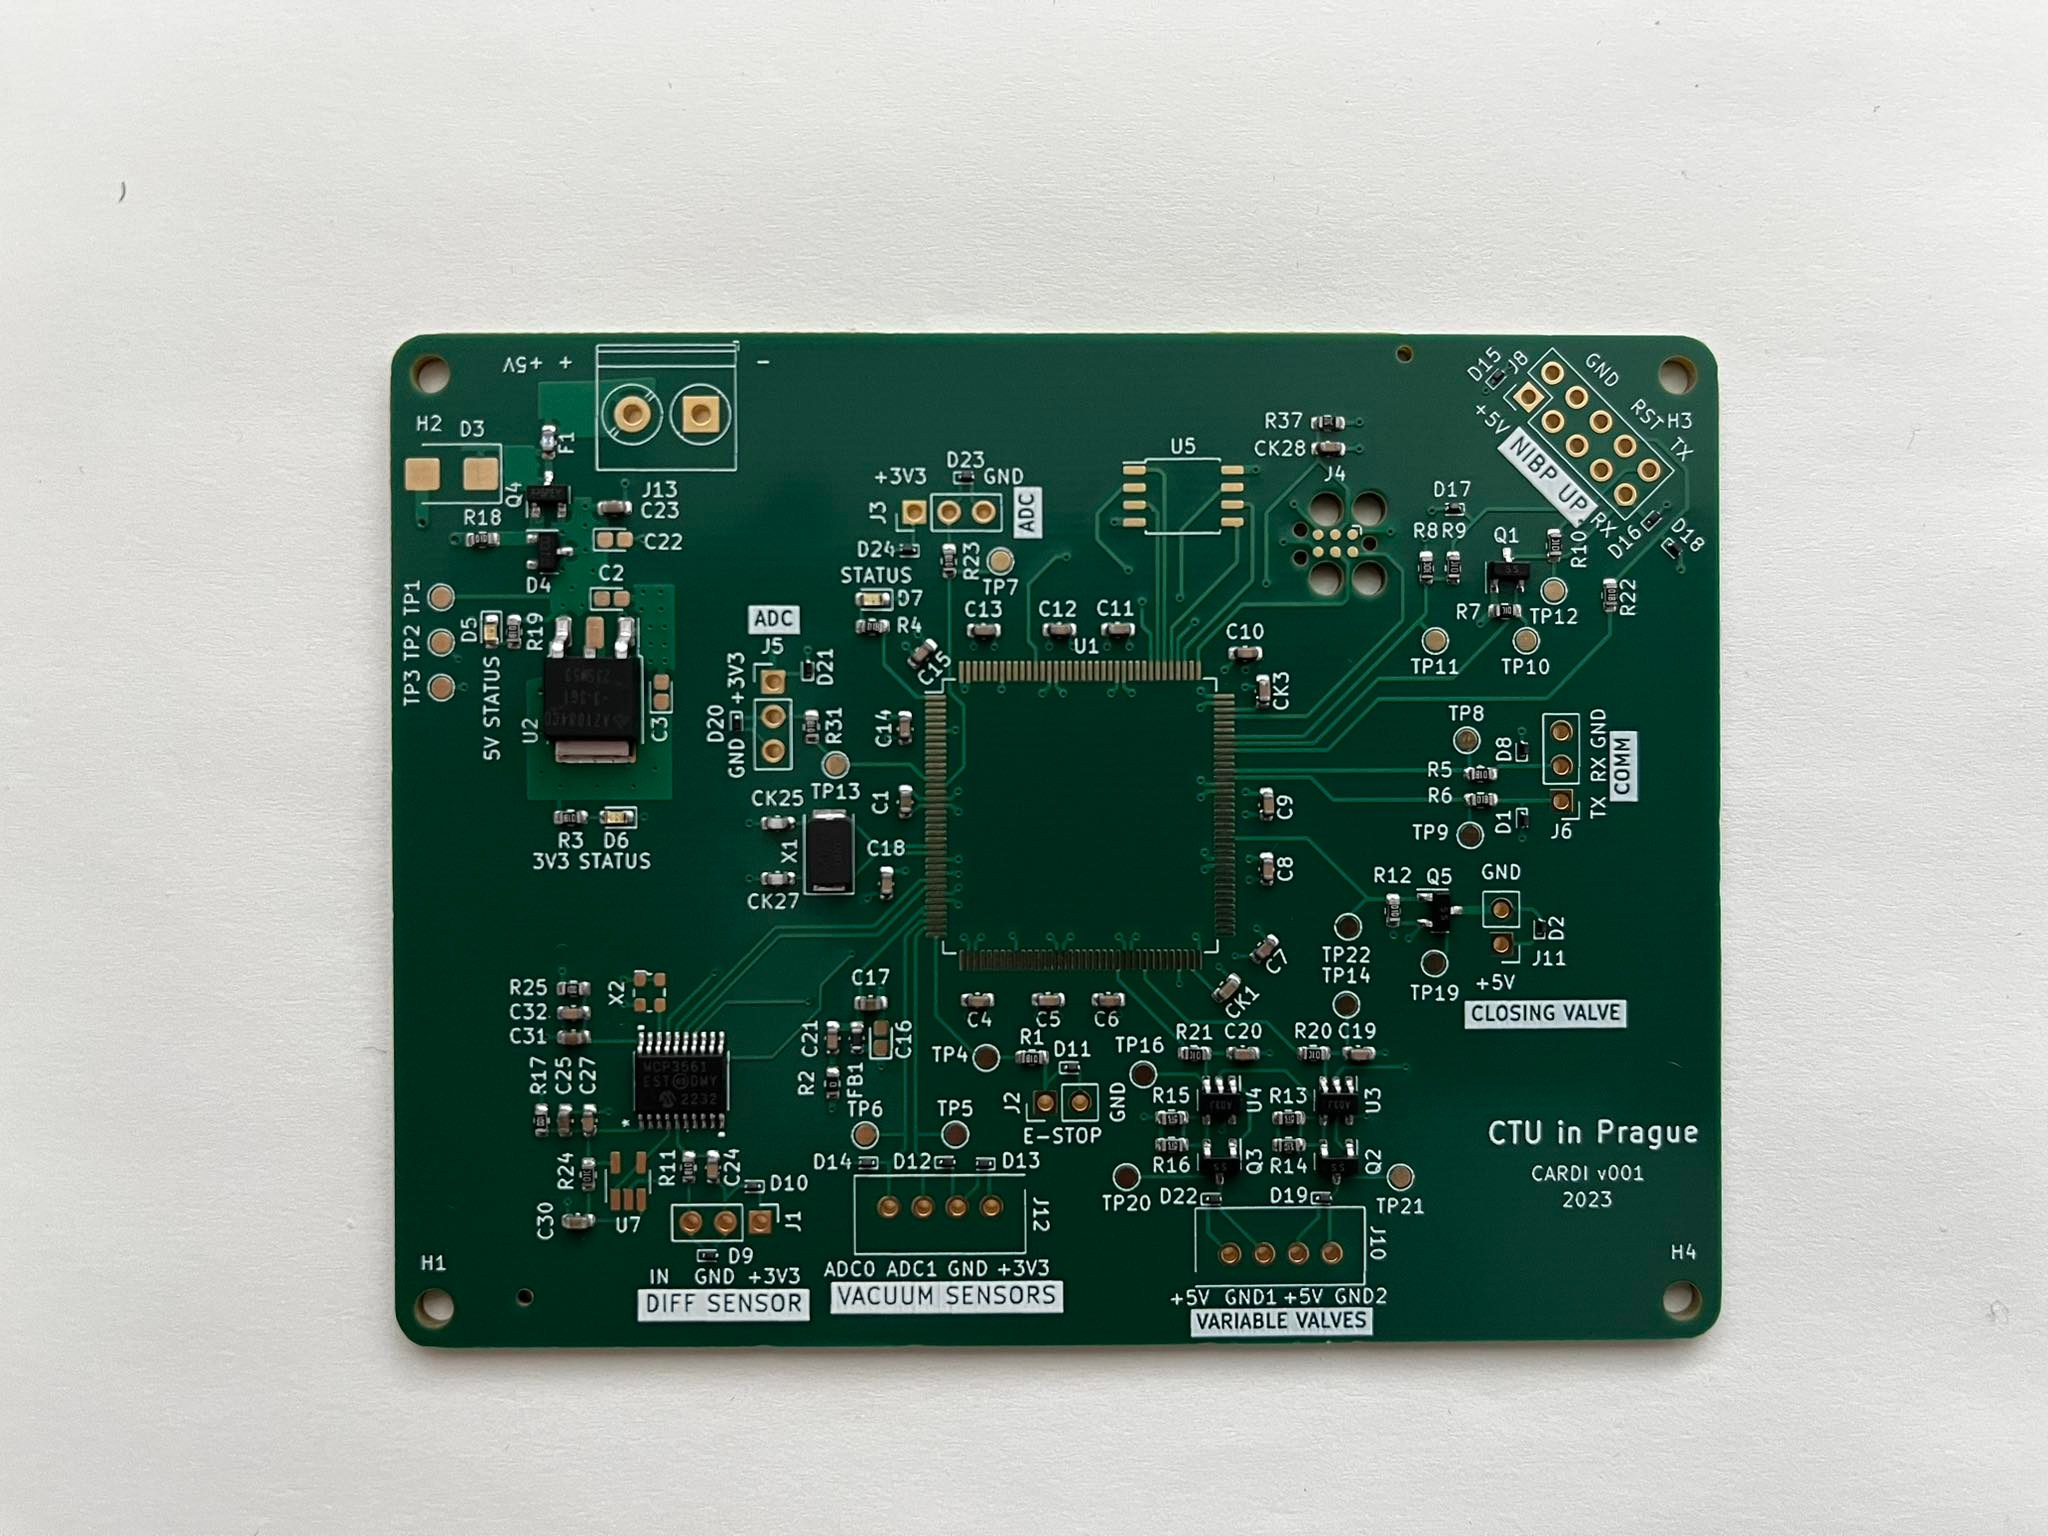
\includegraphics[width=0.9\linewidth]{pictures/pcb_from_production.jpg}
    \caption{Horní pohled desky plošného spoje z výroby.}
    \label{fig:pcb_production}
\end{figure}
\begin{figure}[H]
    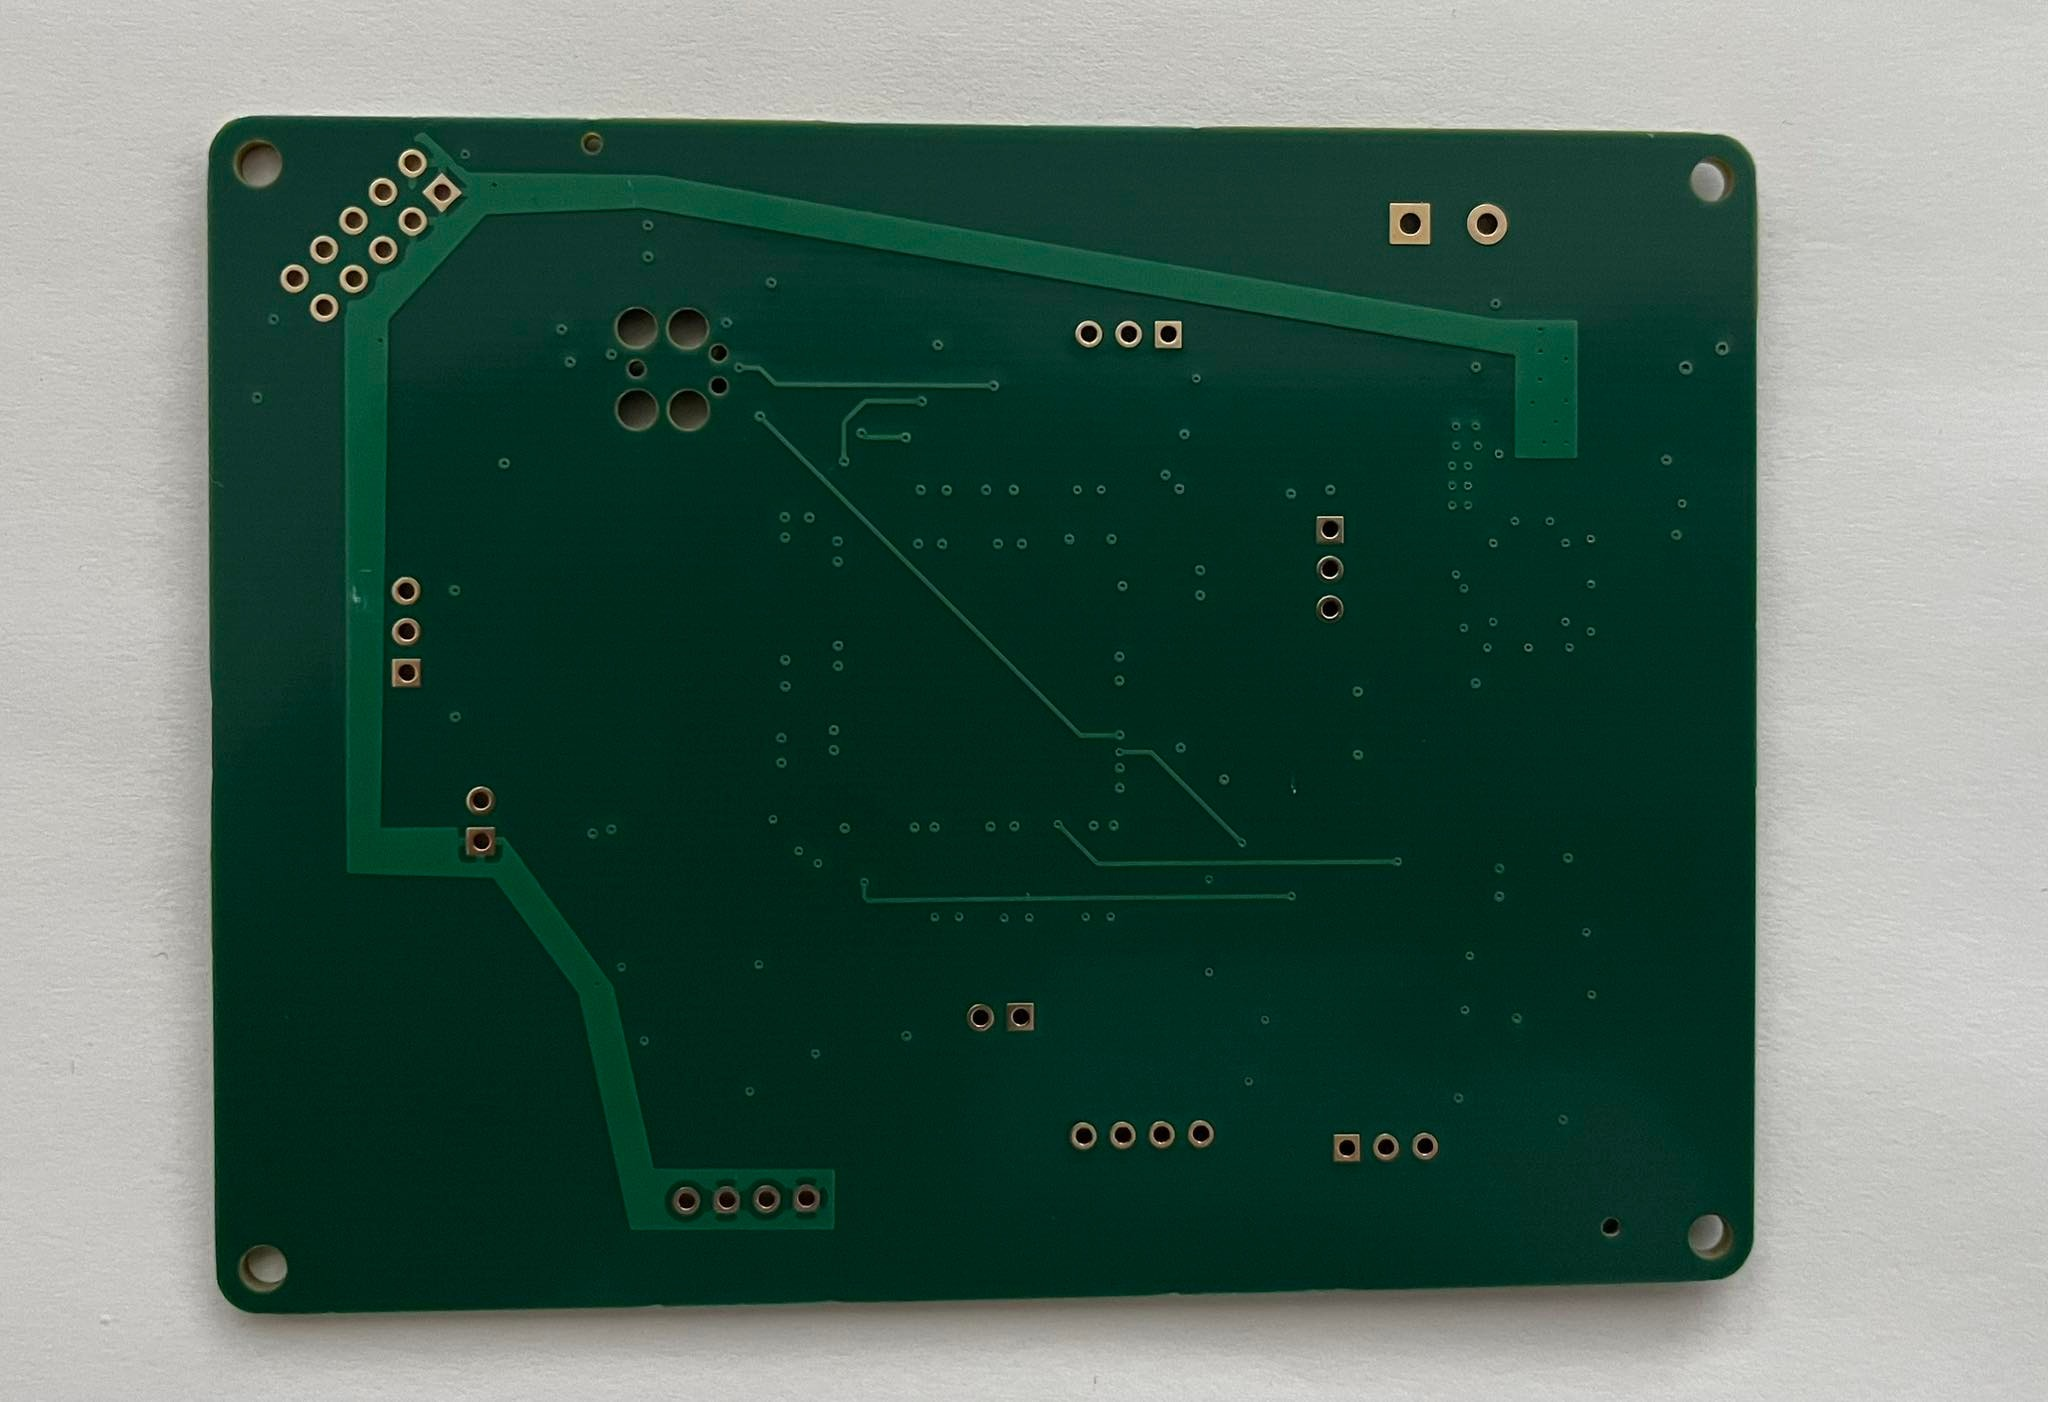
\includegraphics[width=0.9\linewidth]{pictures/pcb_production_bottom.jpg}
    \caption{Spodní pohled desky plošného spoje z výroby.}
    \label{fig:pcb_production_bottom}
\end{figure}

Celková cena DPS a potřebné materiály jsou v níže uvedené tabulce
\begin{table}[H]
    \label{tab:bom}
    \caption{Celkový počet součástek a výrobní cena }
    \hspace*{-1.55cm}
    \begin{ctucolortab}
        \begin{tabular}{ccccccc}
            \toprule
            Typ                   & Název                  & Hodnota       & Počet & Cena     & Jednotky & \\ \midrule
            Kondenzátor           &                        & 100 nF        & 10    & 0.022    &          & \\
            Kondenzátor           &                        & 22 pF         & 2     & 0.0174   &          & \\
            Kondenzátor           &                        & 1 uF          & 4     & 0.018    &          & \\
            Kondenzátor           &                        & 2.2 uF        & 2     & 0.0096   &          & \\
            Kondenzátor           &                        & 4.7 uF        & 1     & 0.0091   &          & \\
            Kondenzátor           &                        & 10 uF         & 1     & 0.006    &          & \\
            Kondenzátor           &                        & 22 uF         & 3     & 0.015    &          & \\
            Rezistor              &                        & 51 $\Omega$   & 4     & 0.5688   &          & \\
            Rezistor              &                        & 10 $\Omega$   & 2     & 0.0032   &          & \\
            Rezistor              &                        & 20 $k\Omega$  & 5     & 0.005    &          & \\
            Rezistor              &                        & 10 $k\Omega$  & 7     & 0.0056   &          & \\
            Rezistor              &                        & 0 $\Omega$    & 1     & 0.001    &          & \\
            Rezistor              &                        & 1 $k\Omega$   & 10    & 0.005    &          & \\
            Rezistor              &                        & 100 $k\Omega$ & 2     & 0.002    & €        & \\
            Dioda                 & BZX84C10VLT116         &               & 1     & 0.2264   &          & \\
            Dioda                 & D5V0F1U2S9-7           &               & 19    & 3.0837   &          & \\
            Dioda                 & SM6T6V8AY              &               & 1     & 0.1372   &          & \\
            Dioda                 & LED Green              &               & 3     & 0.0717   &          & \\
            IO                    & AZ1084CD-3.3TRG1       &               & 1     & 0.2395   &          & \\
            IO                    & MCP3561-E/ST           &               & 1     & 5.5941   &          & \\
            IO                    & MCP6001RT-I/OT         &               & 2     & 0.486    &          & \\
            IO                    & MCP6V91T-E/OT          &               & 1     & 1.81     &          & \\
            IO                    & MX25R3235FM2IL0        &               & 1     & 0.88     &          & \\
            IO                    & STM32F407ZGT6          &               & 1     & 1.02     &          & \\
            MOSFET                & TPM9305PS3-1           &               & 1     & 0.0958   &          & \\
            MOSFET                & BSS138                 &               & 4     & 0.09     &          & \\
            Ferritový korálek     & MPZ1608S102ATA00       &               & 1     & 0.0196   &          & \\
            Oscilátor             & ABM3-8.000MHZ-D2Y-T    & 8 MHz         & 1     & 0.5783   &          & \\
            Oscilátor             & ECS-2520MVLC-049       & 4.9152 MHz    & 1     & 1.23     &          & \\
            Pojistka              & F0603FF4000V032TM      & 4 A           & 1     & 0.0762   &          & \\
            \bottomrule
            $\Sigma$              &                        &               & 94    & 16.3262  & €        & \\
            \bottomrule
            Služba                & Výroba DPS od JLCPCB   &               & 1     & 5        & €        & \\
            Služba                & Osazení DPS od JLCPCB  &               & 1     & 16       & €        & \\
            \bottomrule
            $\Sigma$              &                        &               & 2     & 21       & €        & \\
            \bottomrule
            Programátor           & ST-LINK/V2-ISOL        &               & 1     & 76.99    & €        & \\
            Kabel na programování & Tag Connect TC2030 IDC &               & 1     & 40.37    & €        & \\
            \bottomrule
            $\Sigma$              &                        &               & 2     & 117.36   & €        & \\
            \bottomrule
            \bottomrule
            $\Sigma$              & Bez DPH                &               &       & 154.6862 & €        & \\
            \bottomrule
        \end{tabular}
    \end{ctucolortab}
\end{table}
\section{Pneumatická část}
Pneumatická část systému je část, ve které probíhá měření hemodynamických parametrů srdce pacienta a je sestavena podle patentu \cite[US Patent US10251567]{cite:2}.

\begin{figure}[H]
    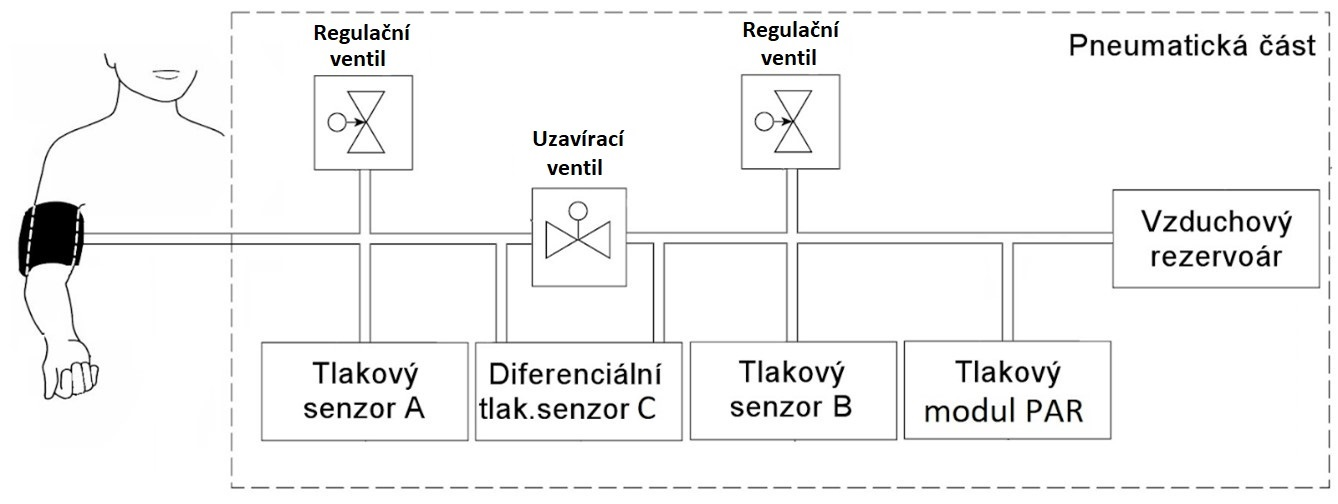
\includegraphics[width=1\linewidth]{pictures/blokove_schema_pneu.jpg}
    \caption{Blokové schéma pneumatického systému}
    \label{fig:pneu_block}
\end{figure}
\subsection{Metoda měření} \label{section:metoda_mereni}
Měření probíhá ve dvou fázích, v první fázi se systém natlakuje na suprasystolický tlak $P_s$ při otevřeném uzavíracím ventilu a zavřených regulačních ventilech, kde suprasystolický tlak $P_s$ je $\approx 50 \ mmHg$ nad systolickým tlakem pacienta.
\begin{figure}[H]
    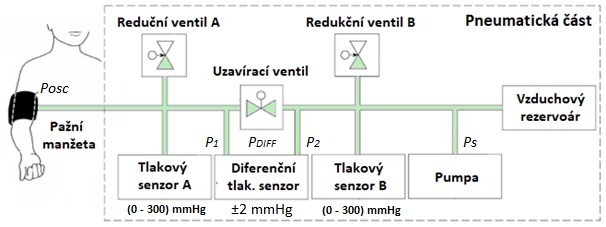
\includegraphics[width=1\linewidth]{pictures/faze_mereni_1.jpg}
    \caption{První fáze měření oscilometrických pulzací \cite{cite:Habilitace}}
\end{figure}
V celé pneumatické části bude suprasystolický tlak a tlak v jednotlivých bodech je
\begin{equation*}
    P_1 = P_{osc} + P_s
\end{equation*}
\begin{equation*}
    P_2 = P_{osc} + P_s
\end{equation*}
\begin{equation*}
    P_{DIFF} = P_1 - P_2 = 0
\end{equation*}
Na výstupu diferenčního sensoru tlaku je nulový signál. \par
V druhé fázi měření po natlakování systému na suprasystolický tlak se uzavře uzavírací ventil.
\begin{figure}[H]
    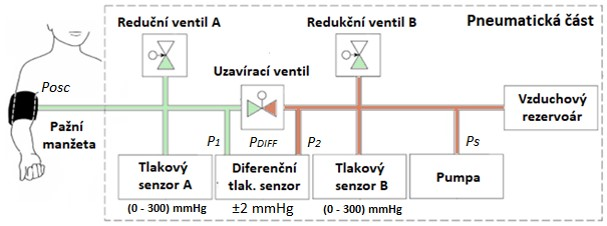
\includegraphics[width=1\linewidth]{pictures/faze_mereni_2.jpg}
    \caption{Druhá fáze měření oscilometrických pulzací \cite{cite:Habilitace}}
\end{figure}
Tlak na větvích pneumatického systému bude následovný
\begin{equation*}
    P_1 = P_{osc} + P_s
\end{equation*}
\begin{equation*}
    P_2 = P_s
\end{equation*}
\begin{equation}
    P_{DIFF} = P_1 - P_2 = P_{osc}
\end{equation}
Jelikož měříme rozdíl tlaků ve větvích, na výstupním signálu diferenčního sensoru budou pouze tlakové oscilace $P_{osc}$.
Pomocí regulačních ventilů se bude snižovat statický tlak v obou větví současně, aby nadále zůstala pouze oscilační složka.
Tento způsob měření způsobí zvýšení citlivosti snímání tlakových pulzací pomocí diferenčního sensoru tlaku 75x až 150x. \cite{cite:Habilitace}
Metoda je patentována v České Republice a USA \cite{cite:2} a splňuje kritéria normy ISO 81060–2:2013 \cite{cite:Validation}.
\pagebreak
\subsection{Měření těsnosti penumatické části}
Pneumatická část musí být co nejlépe těsná, aby po dobu měření byl co nejmenší úbytek tlaku v systému.
\par
Test těsnosti probíhal pomocí přístroje FLUKE Biomedical BP pump 2, který natlakoval pneumatickou část na hodnotu 200 $mmHg$ a následně sledoval úbytek tlaku v systému po dobu 60 s.
Měření bylo opakováno 10 krát po sobě.

\begin{table}[H]
    \label{tab:pressure_test_pneu}
    \caption{Test těsnosti pneumatického systému}
    \begin{ctucolortab}
        \begin{tabular}{ccc}
            \toprule
            Měření & Těsnost & Jednotky           \\ \midrule
            1      & 0.9     &                    \\
            2      & 0.8     &                    \\
            3      & 1.1     &                    \\
            4      & 1.0     &                    \\
            5      & 0.9     & $\frac{mmHg}{min}$ \\
            6      & 0.9     &                    \\
            7      & 1.1     &                    \\
            8      & 0.9     &                    \\
            9      & 0.8     &                    \\
            10     & 1.0     &                    \\
            \bottomrule
        \end{tabular}
    \end{ctucolortab}
\end{table}
Průměrný pokles tlaku v důsledku úniku vzduchu z pneumatického obvodu je $\mu = 0.94 \ \frac{mmHg}{min}$ se směrodatnou odchylkou $\sigma = 0.10  \ \frac{mmHg}{min}$.
Dle normy ISO 81060–1:2013 maximální úbytek tlaku v systému nesmí přesahovat $P_{loss} = 6 \ \frac{mmHg}{min}$.
\pagebreak
\subsection{Zkreslení signálu pneumatickým systémem}
Přenosová funkce systému byla identifikována měřením impulzní odezvy systému. Systém byl natlakován na průměrnou hodnotu suprasystolického tlaku $230 mmHg$ a poté
byl aplikován jednotkový impuls pomocí mechanického kyvadla. \cite{cite:Patricia}
\begin{figure}[H]
    \label{fig:mech_kyvadlo}
    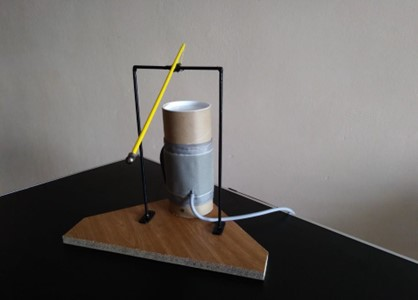
\includegraphics[width=1\textwidth]{pictures/mech_kyvadlo.jpg}
    \caption{Mechanické kyvadlo pro vytvoření jednotkového impulsu na pneumatický systém. \cite{cite:Patricia}}
\end{figure}
\begin{figure}[H]
    \label{fig:pneu_impulse_response}
    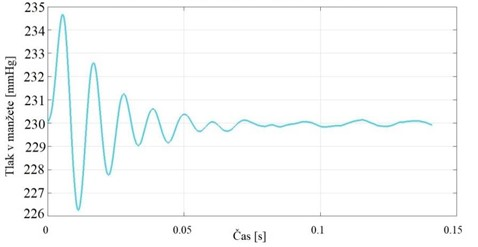
\includegraphics[width=1\textwidth]{pictures/pneu_impulse.jpg}
    \caption{Odezva pneumatického systému na jednotkový impuls. \cite{cite:Patricia}}
\end{figure}
Z naměřené hodnoty impulzní odezvy byly vypočteny parametry vlastní frekvence $f_0 \ [Hz]$ a poměrného útlumu $\xi \ [-]$. Pomocí těchto parametrů, za předpokladu, že se jedná o dynamický systém druhého řádu, bylo možné vypočítat přenosovou funkci systému.\cite{cite:Patricia}
\begin{figure}[H]
    \caption{Odezva pneumatického systému na jednotkový impuls. \cite{cite:Patricia}}
    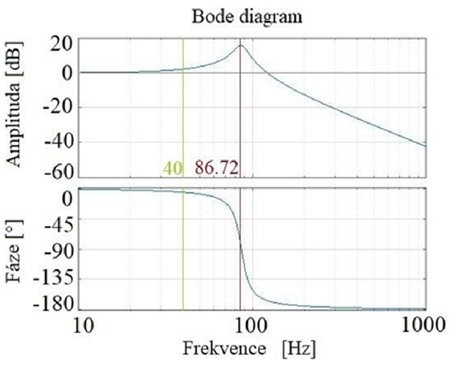
\includegraphics[width=1\textwidth]{pictures/freq_char_pneu.png}
    \label{fig:pneu_freq_char}
\end{figure}
Při měření srdečních frekvencí např. 120 tepů/min tj. 2 Hz, odpovídá 20. harmonická složka tepu frekvenci $f = 40 \ Hz$. Podle obrázku (\ref{fig:pneu_freq_char}) srdeční frekvence je amplituda zkreslena o +2 dB a fáze signálu o $^\circ 5$ \cite{cite:Patricia}, což jsou akceptovatelné hodnoty.

%
%
%
%
\pagebreak
\section{Vyhodnocení dat z AD převodníků}
Tato sekce se zaměří o popsání charakteristiky 12bitového AD převodníku a 24bitového AD převodníku MCP3561. Měření probíhalo na třech veličinách, vstupní piny byly zkratovány s referenční zemí, na napětí z DPS $U_{ref} = 3.3 \ V$ a poté pomocí napěťového děliče ze $U_{ref}$ na $U_{h} = 1.63 \ V$.
Všechny součástky a referenční hodnoty měření jsou napájené z napájecího napětí na DSP při hodnotě $3.3 \ V$ kde reálná hodnota je $U_{ref} = 3.29 \ V$. Během měření nebyl brán v dotaz fluktuace ambientní teploty, ani teploty samostatných součástek. Dělič napětí pro hodnotu $U_{h} = 1.63 \ V$ bylo provedeno na vedlejším nepájivém poli.

\subsection{Charakteristika 12bitového AD převodníku STM32}
12bitový AD převodník je součástí MCU STM32F407ZGT6. AD převodník slouží k měření absolutní hodnoty tlaku z tlakových sensorů na obou větví pneumatického systému.
Hodnota 1 LSB $= \frac{U_{ref}}{2^{12}} = 802 \ \mu V$.
\begin{figure}[H]
    \caption{Graf počtu hodnot LSB 12bitového AD převodníku při připojení kanálu pro první tlakový sensor k referenční zemi.}
    \label{fig:hist_vacuum1_gnd}
    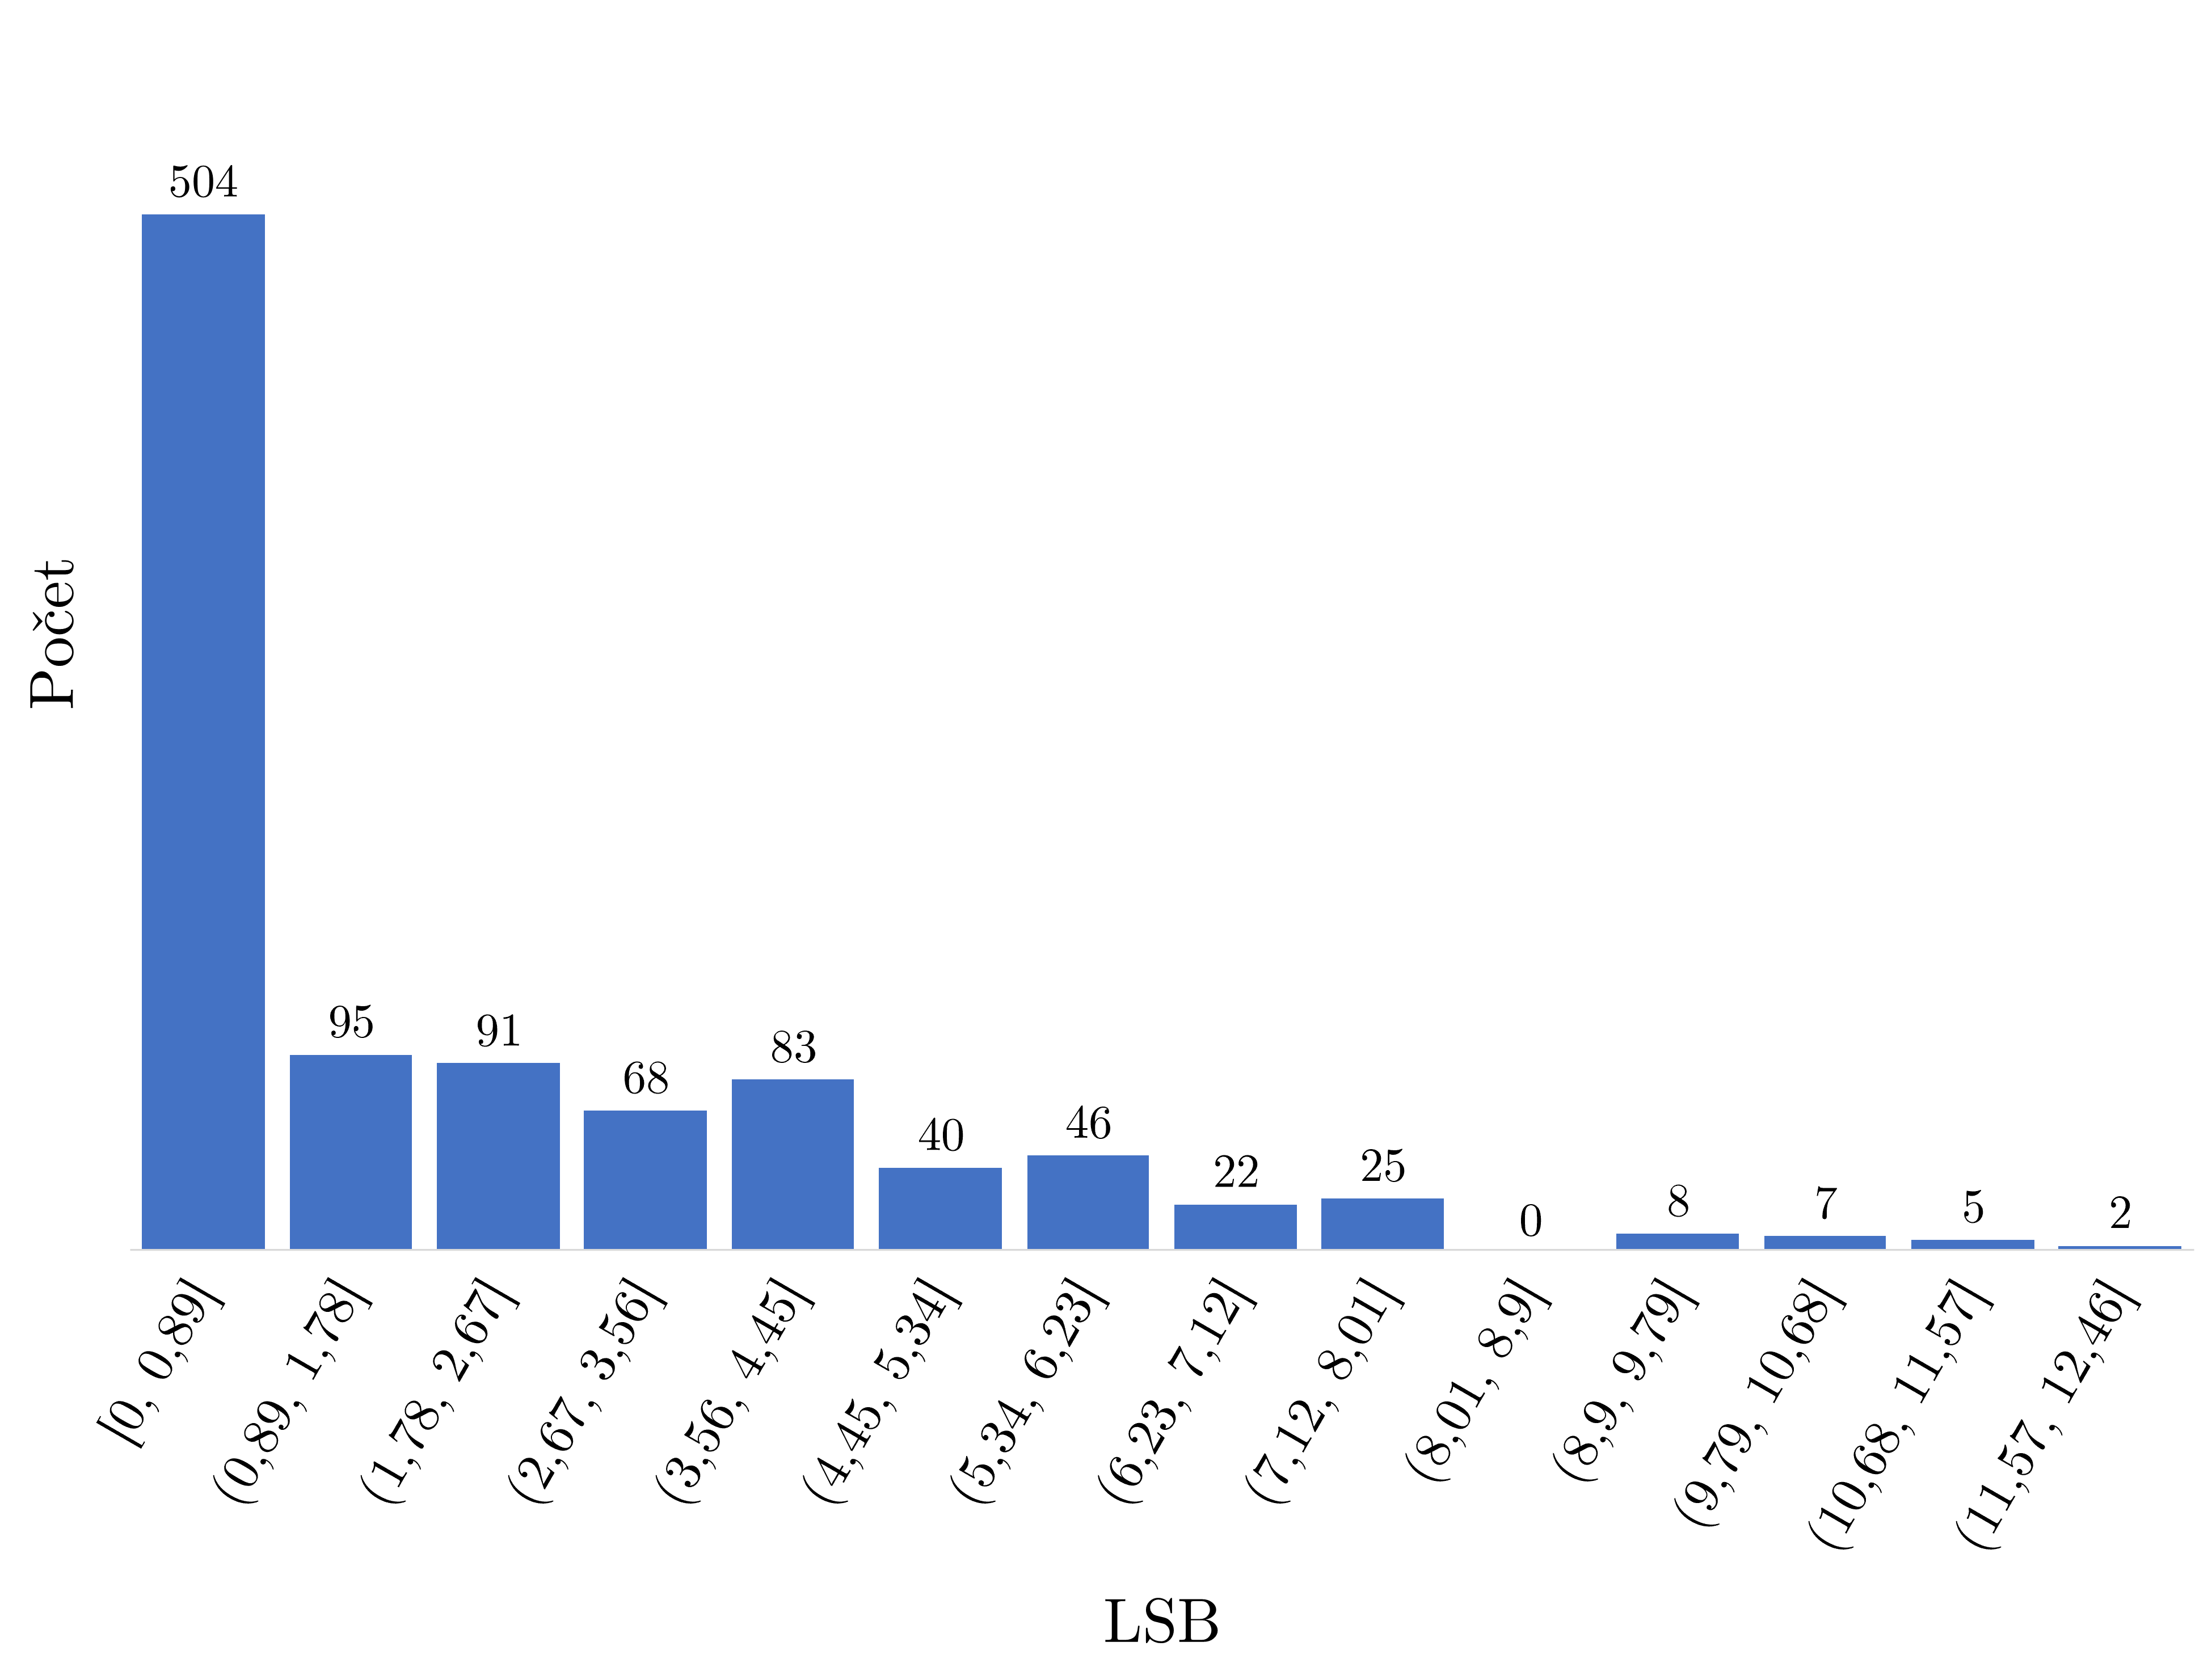
\includegraphics[width=1\textwidth]{graphs/vacuum1_gnd.png}

\end{figure}
Očekáváné hodnoty pro připojení k referenční zemi je 0. Střední hodnota naměřených dat je $\mu = 1.87$ se směrodatnou odchylkou $\sigma = 2.55$. Aktuální hodnoty se liší od čekávané o $U_{offset} = 1.503 \pm 2.05 \ mV$.

\begin{figure}[H]
    \caption{Graf počtu hodnot LSB 12bitového AD převodníku při připojení kanálu pro první tlakový sensor k $1.63 \ V$.}
    \label{fig:hist_vacuum1_1_6}
    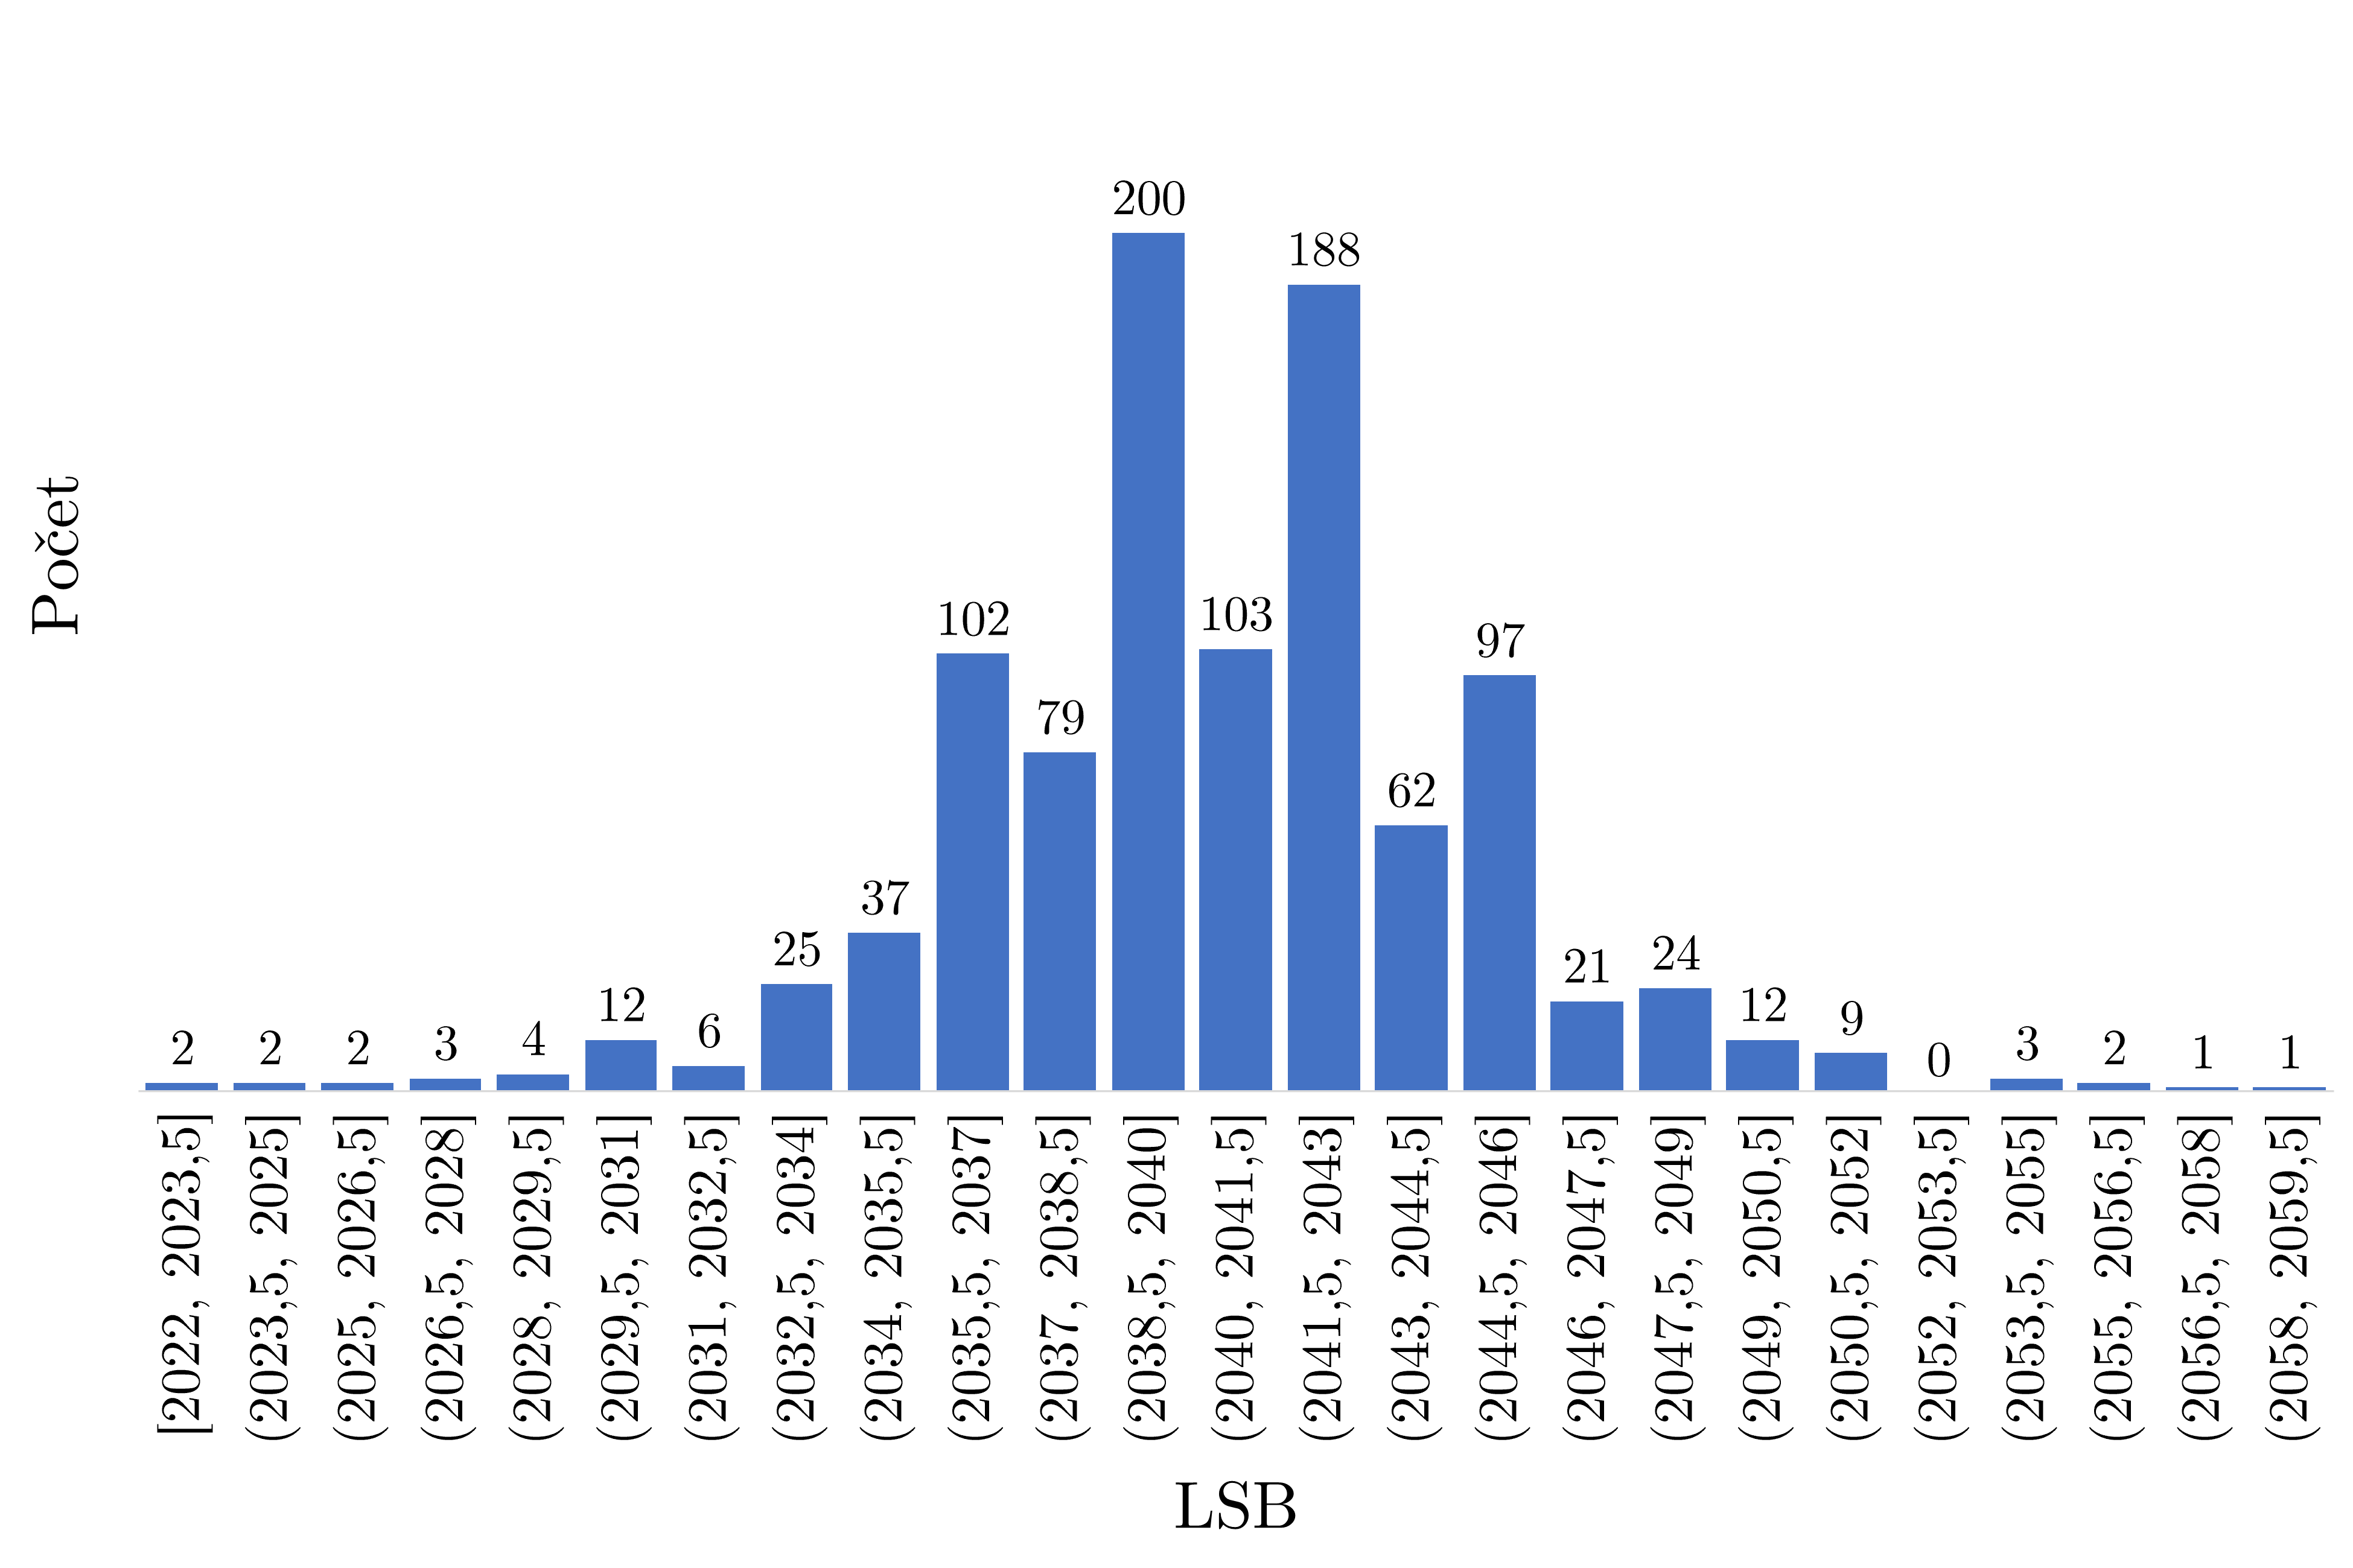
\includegraphics[width=1\textwidth]{graphs/vacuum1_16.png}

\end{figure}

Očekáváné hodnoty pro připojení k $U_{in} = 1.63 \ V$ jsou $2023.17$. Střední hodnota naměřených dat je $\mu = 2036.15$ se směrodatnou odchylkou $\sigma = 4.14$. Po převedení naměřených dat na napětí $U_{out} = 1.63 \pm 0.0033 \ V$ je napěťový rozdíl od očekávané hodnoty $U_{in} = 1.63 \ V$
$U_{offset} = 10.41 \pm 3.32 \ mV$.

\pgfplotstablegetrowsof{graphs/vacuum1_3_3_v.dat}
\begin{figure}[H]
    \caption{Graf počtu hodnot LSB 12bitového AD převodníku při připojení kanálu pro první tlakový sensor k $3.29 \ V$.}
    \label{fig:hist_vacuum1_3_3}
    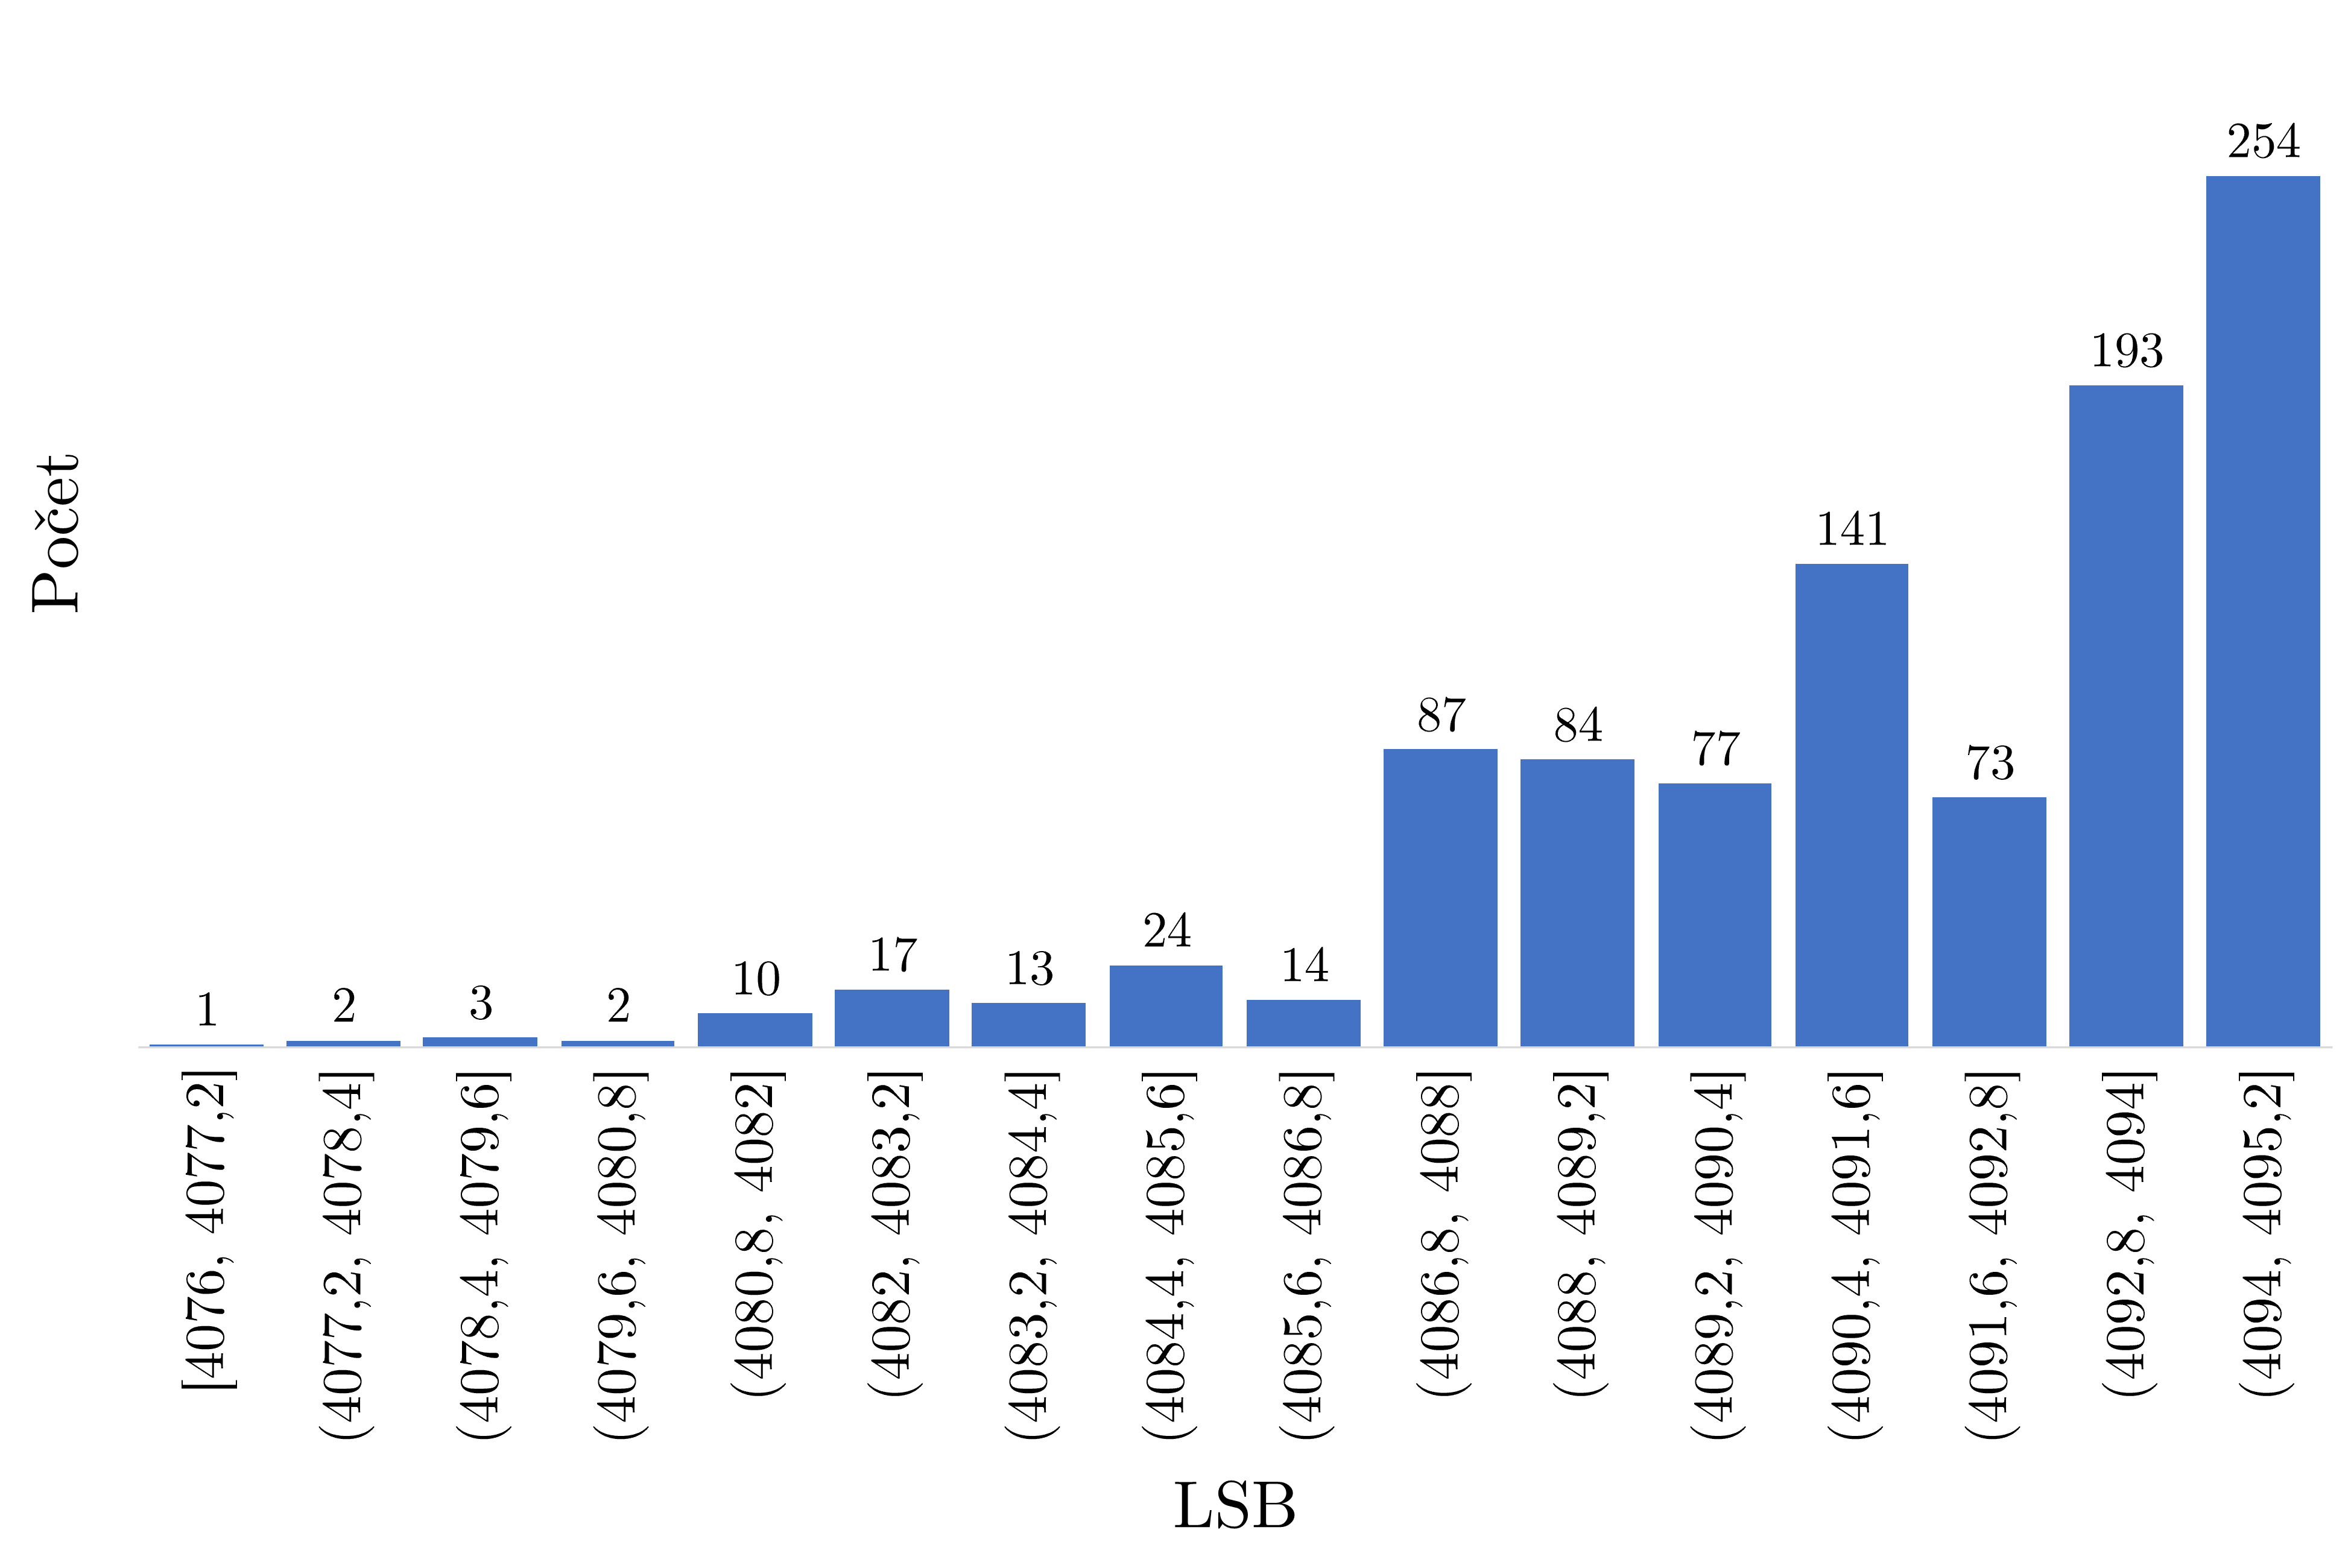
\includegraphics[width=1\textwidth]{graphs/vacuum1_33.png}
\end{figure}

Očekáváné hodnoty pro připojení k $U_{in} = U_{ref} \ V$ jsou $4095$. Střední hodnota naměřených dat je $\mu = 4091.36$ se směrodatnou odchylkou $\sigma = 3.46$. Po převedení naměřených dat na napětí $U_{out} = 3.28 \pm 0.0027 \ V$ je napěťový rozdíl od očekávané hodnoty $U_{in} = U_{ref} = 3.29 \ V$
$U_{offset} = -2.92 \pm 2.78 \ mV$.



\begin{figure}[H]
    \caption{Graf počtu hodnot LSB 12bitového AD převodníku při připojení kanálu pro druhý tlakový sensor k referenční zemi.}
    \label{fig:hist_vacuum2_gnd}
    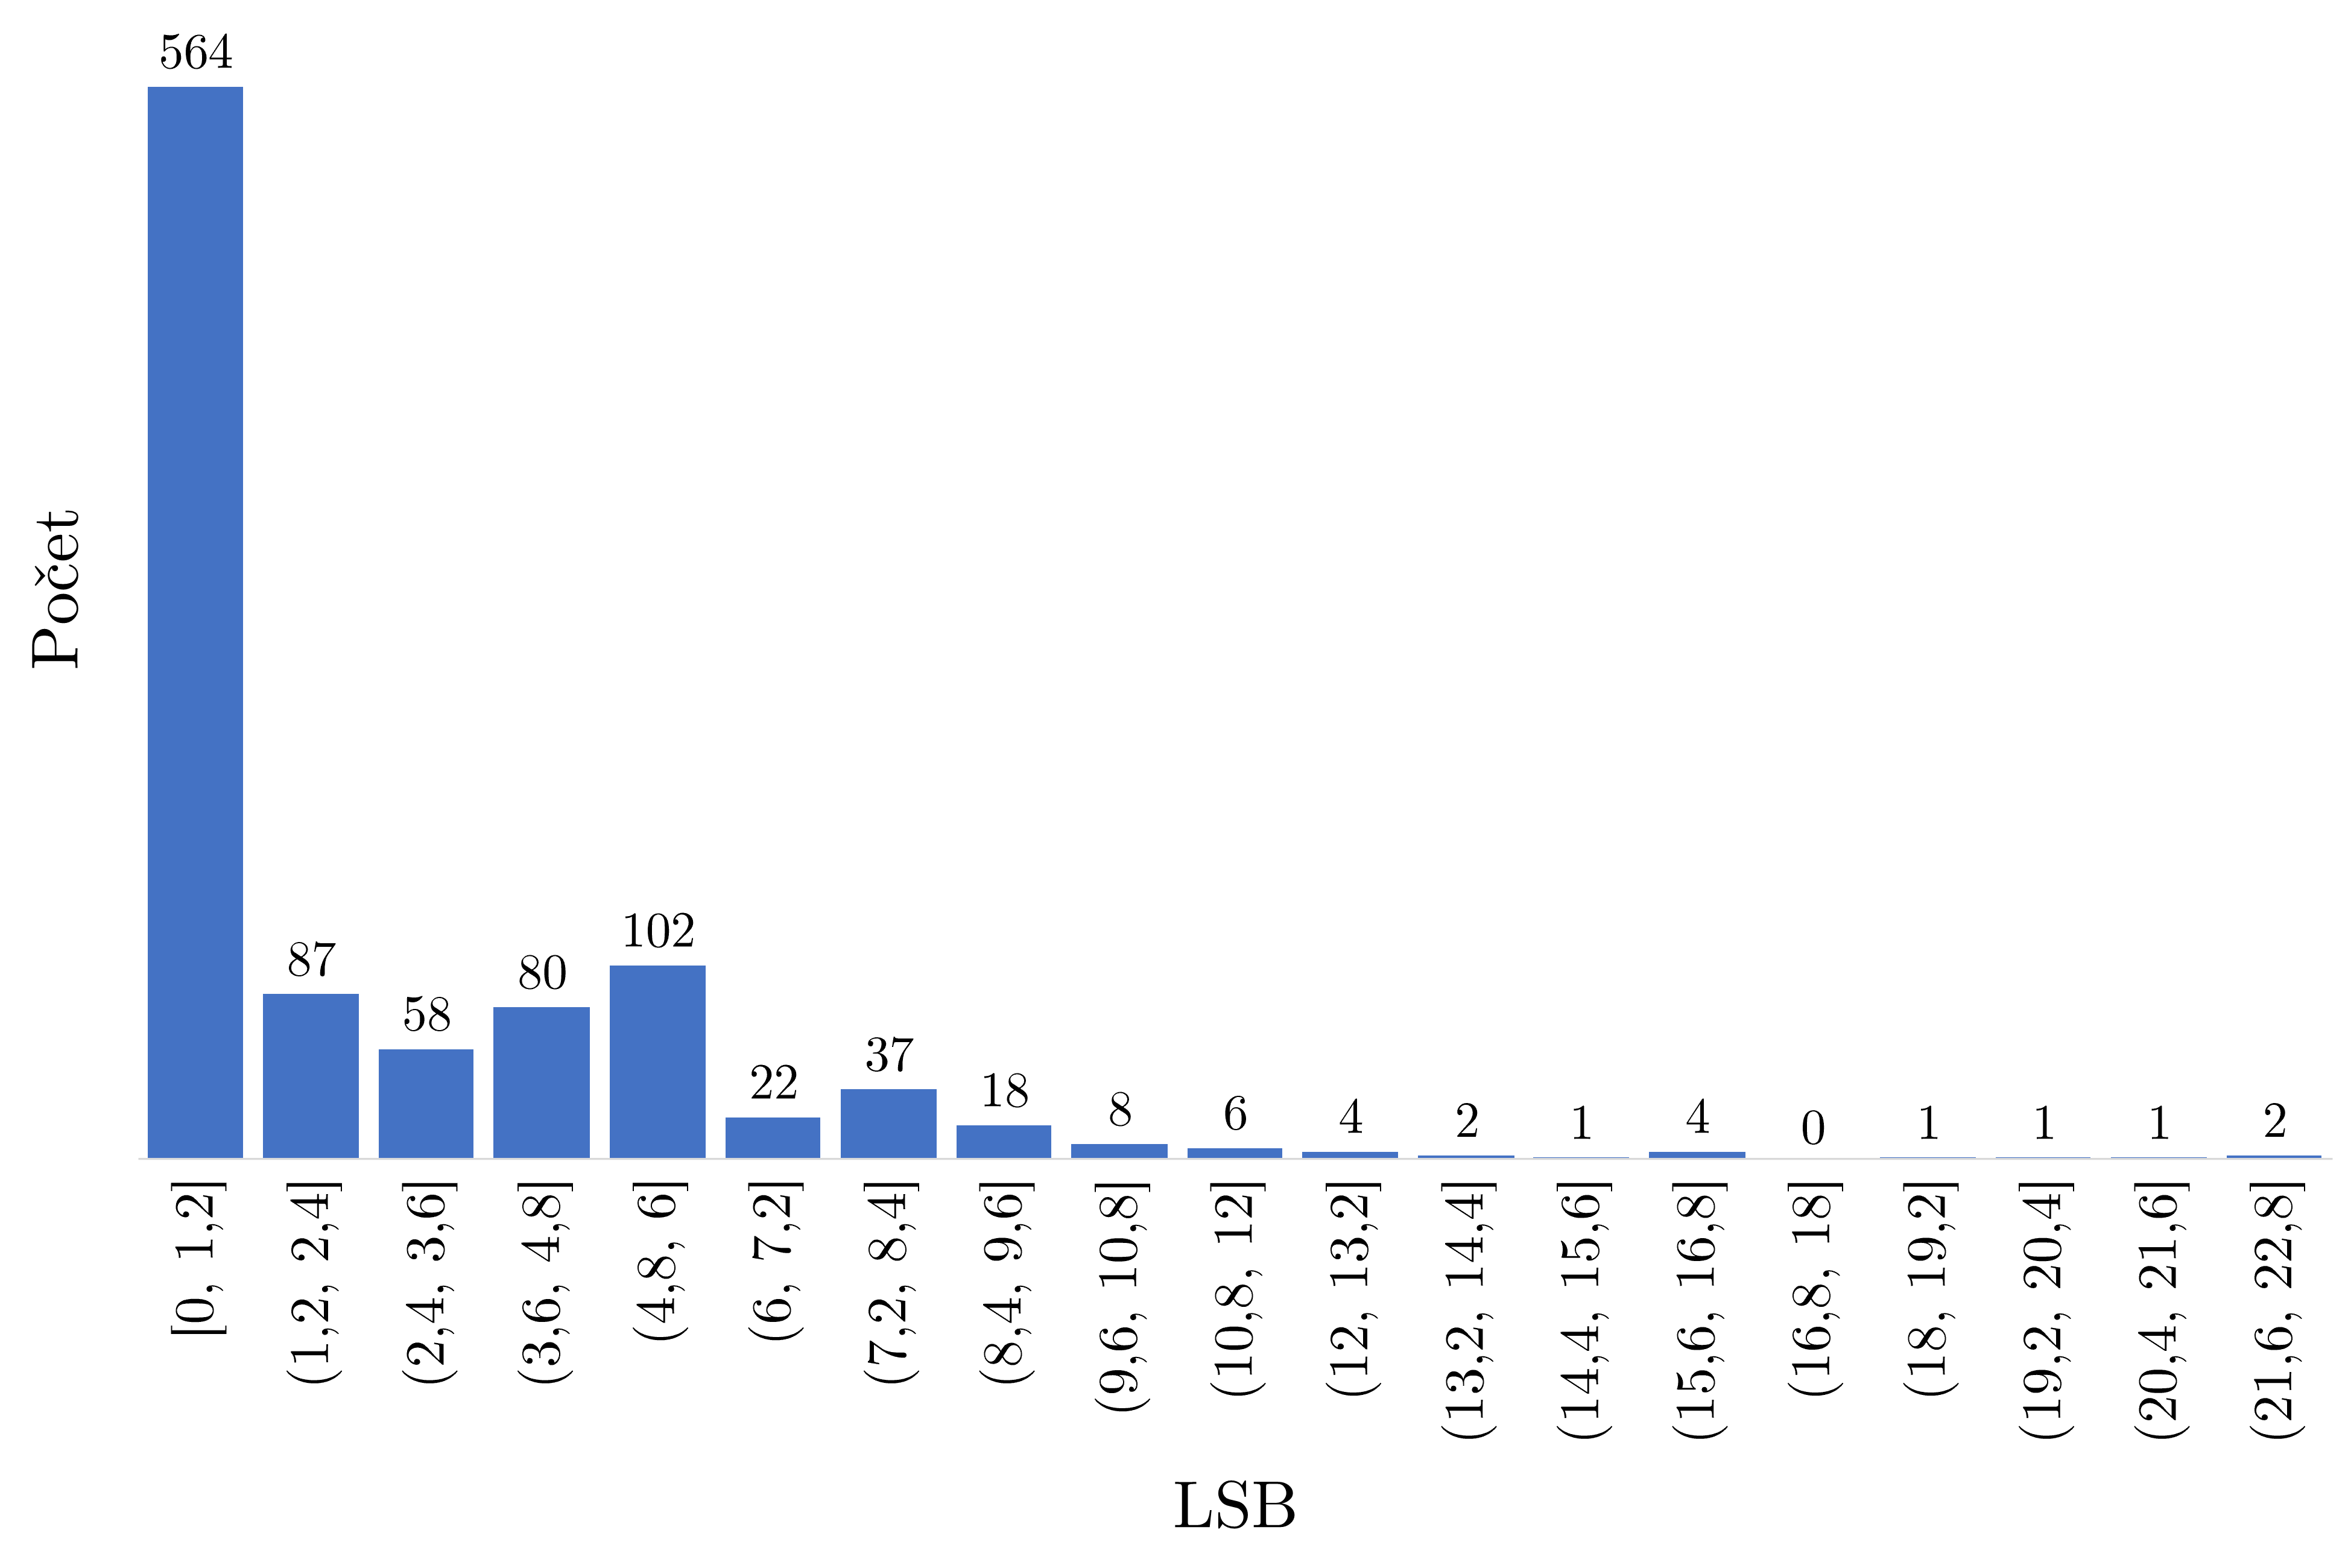
\includegraphics[width=1\textwidth]{graphs/vacuum2_gnd.png}

\end{figure}
Očekáváné hodnoty pro připojení k referenční zemi je 0. Střední hodnota naměřených dat je $\mu = 2.33$ se směrodatnou odchylkou $\sigma = 3.31$. Aktuální hodnoty se liší od čekávané o $U_{offset} = 1.88 \pm 2.66 \ mV$.

\begin{figure}[H]
    \caption{Graf počtu hodnot LSB 12bitového AD převodníku při připojení kanálu pro druhý tlakový sensor k $1.63 \ V$.}
    \label{fig:hist_vacuum2_1_6}
    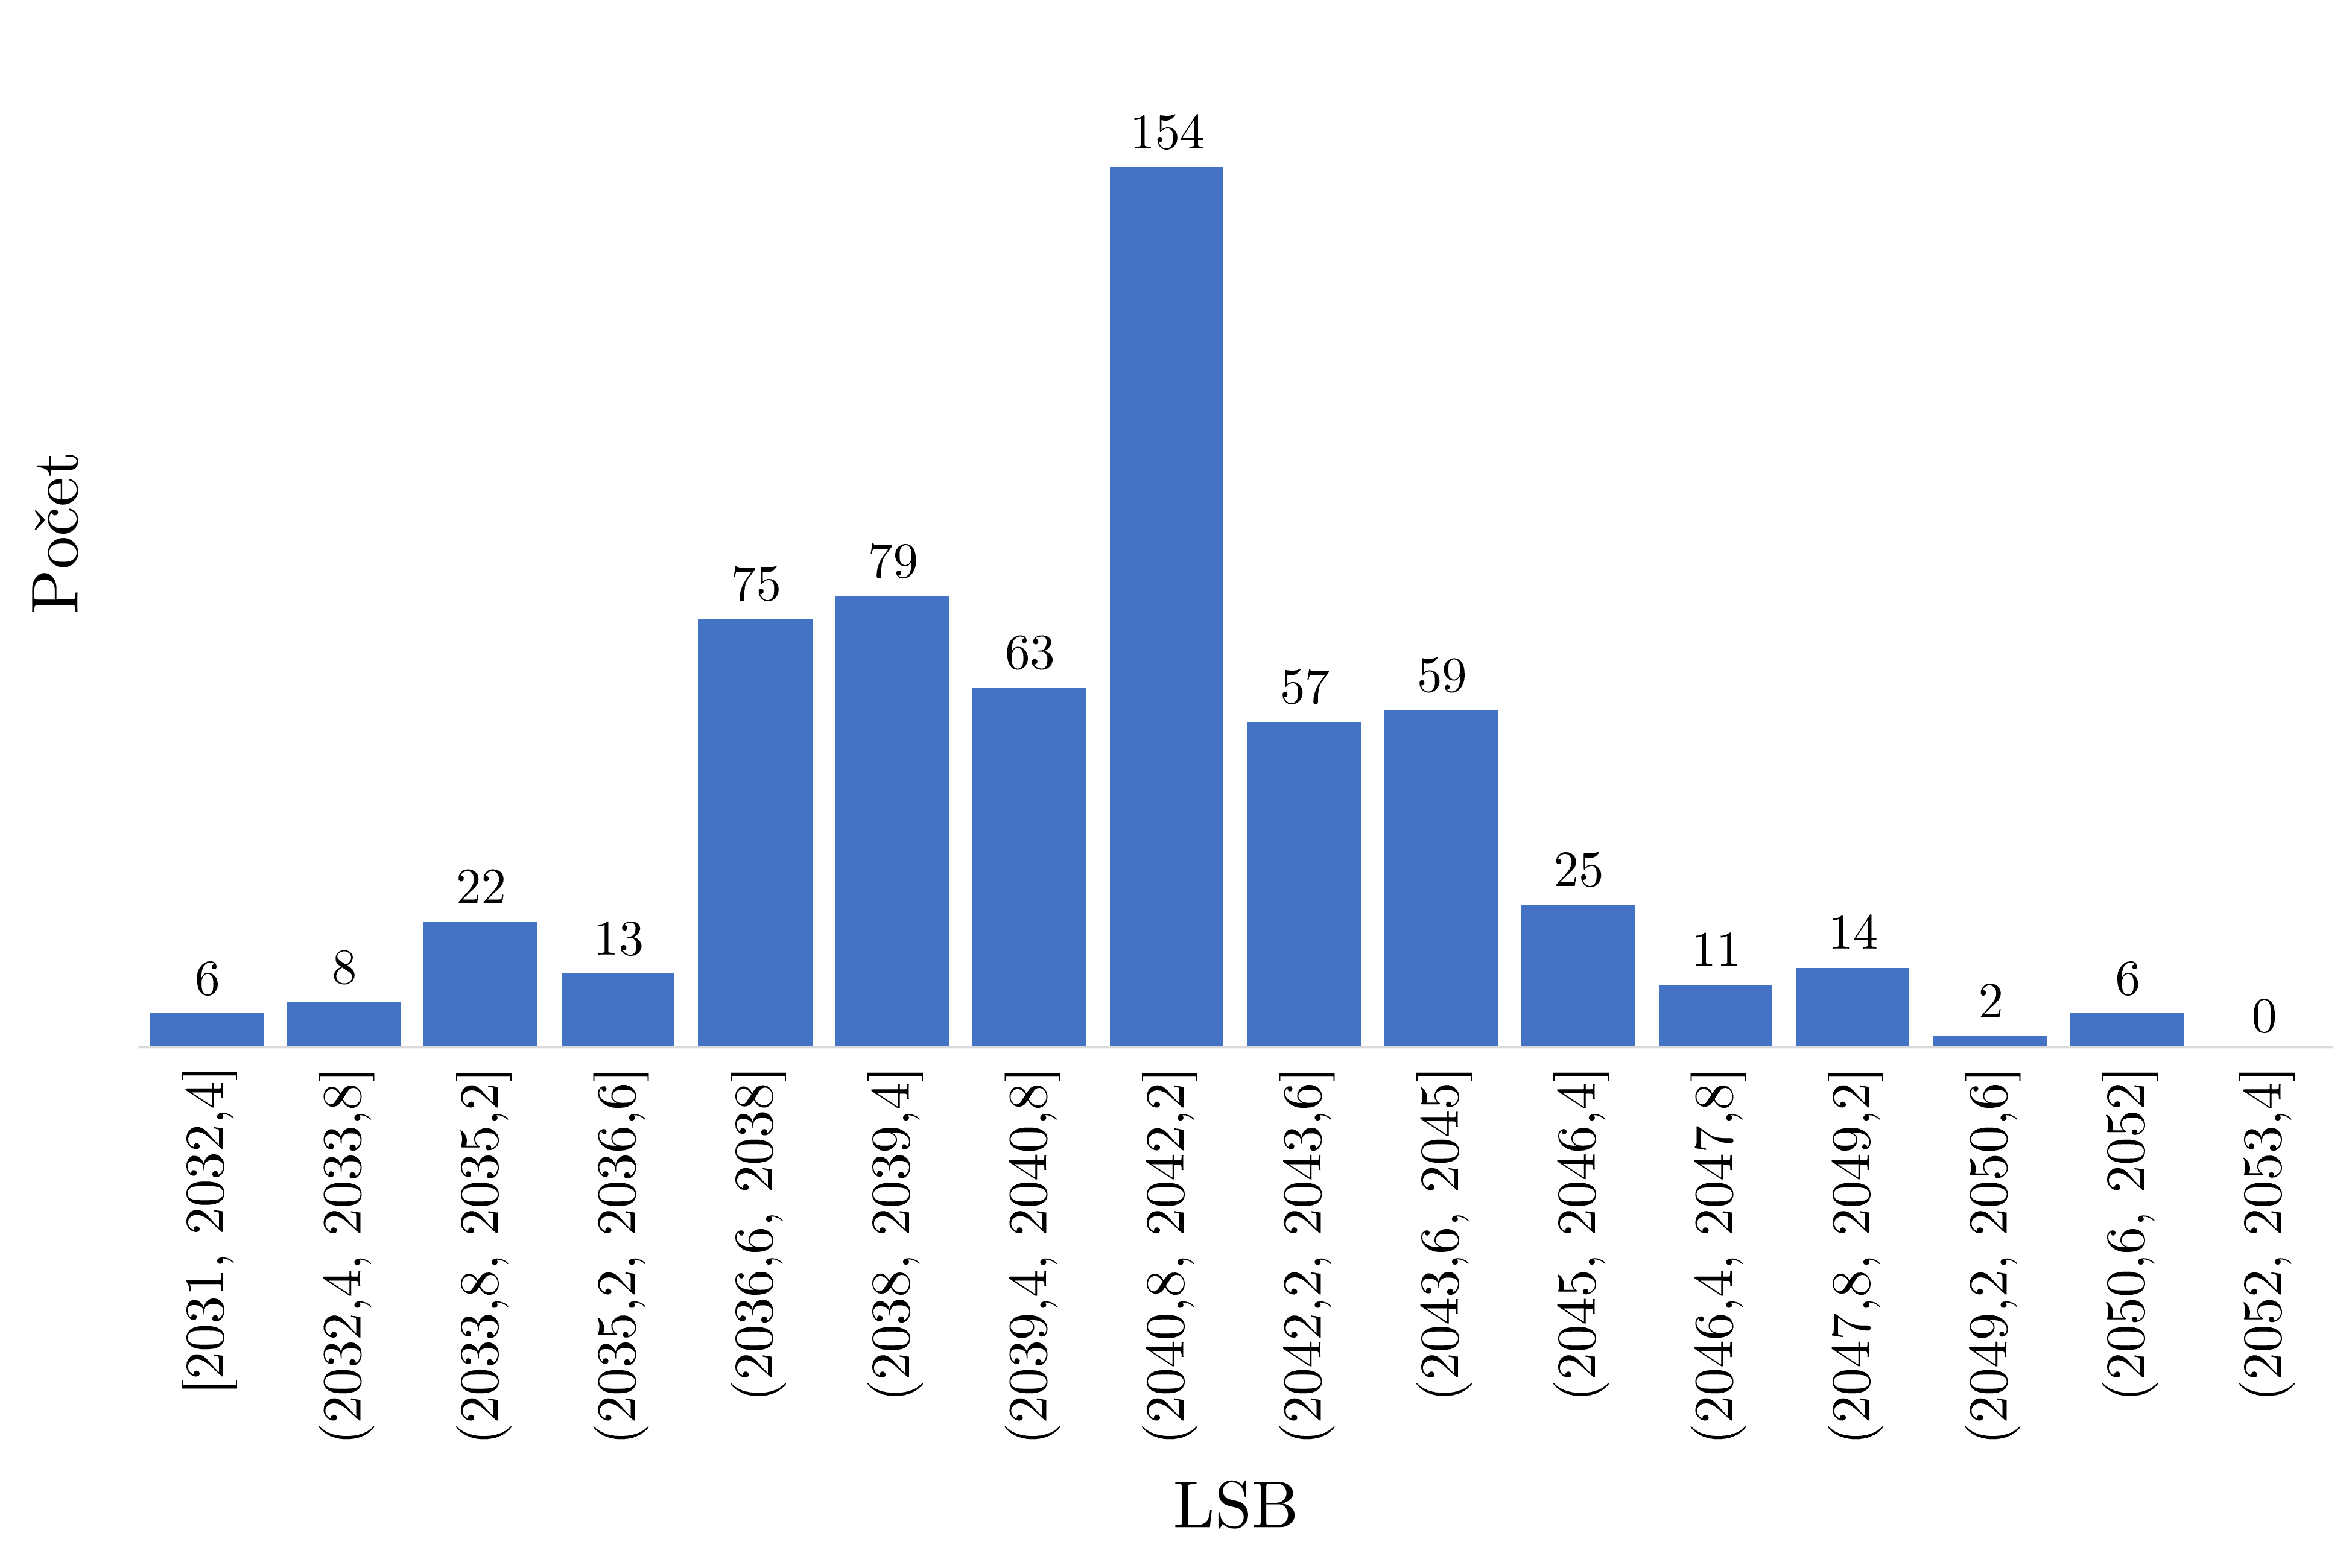
\includegraphics[width=1\textwidth]{graphs/vacuum2_16.png}

\end{figure}
Očekáváné hodnoty pro připojení k $U_{in} = 1.63 \ V$ jsou $2023.17$. Střední hodnota naměřených dat je $\mu = 2036.06$ se směrodatnou odchylkou $\sigma = 7.65$. Po převedení naměřených dat na napětí $U_{out} = 1.63 \pm 0.0061 \ V$ je napěťový rozdíl od očekávané hodnoty $U_{in} = 1.63 \ V$
$U_{offset} = 10.35 \pm 6.15 \ mV$.

\begin{figure}[H]
    \caption{Graf počtu hodnot LSB 12bitového AD převodníku při připojení kanálu pro druhý tlakový sensor k $3.29 \ V$.}
    \label{fig:hist_vacuum2_3_3}
    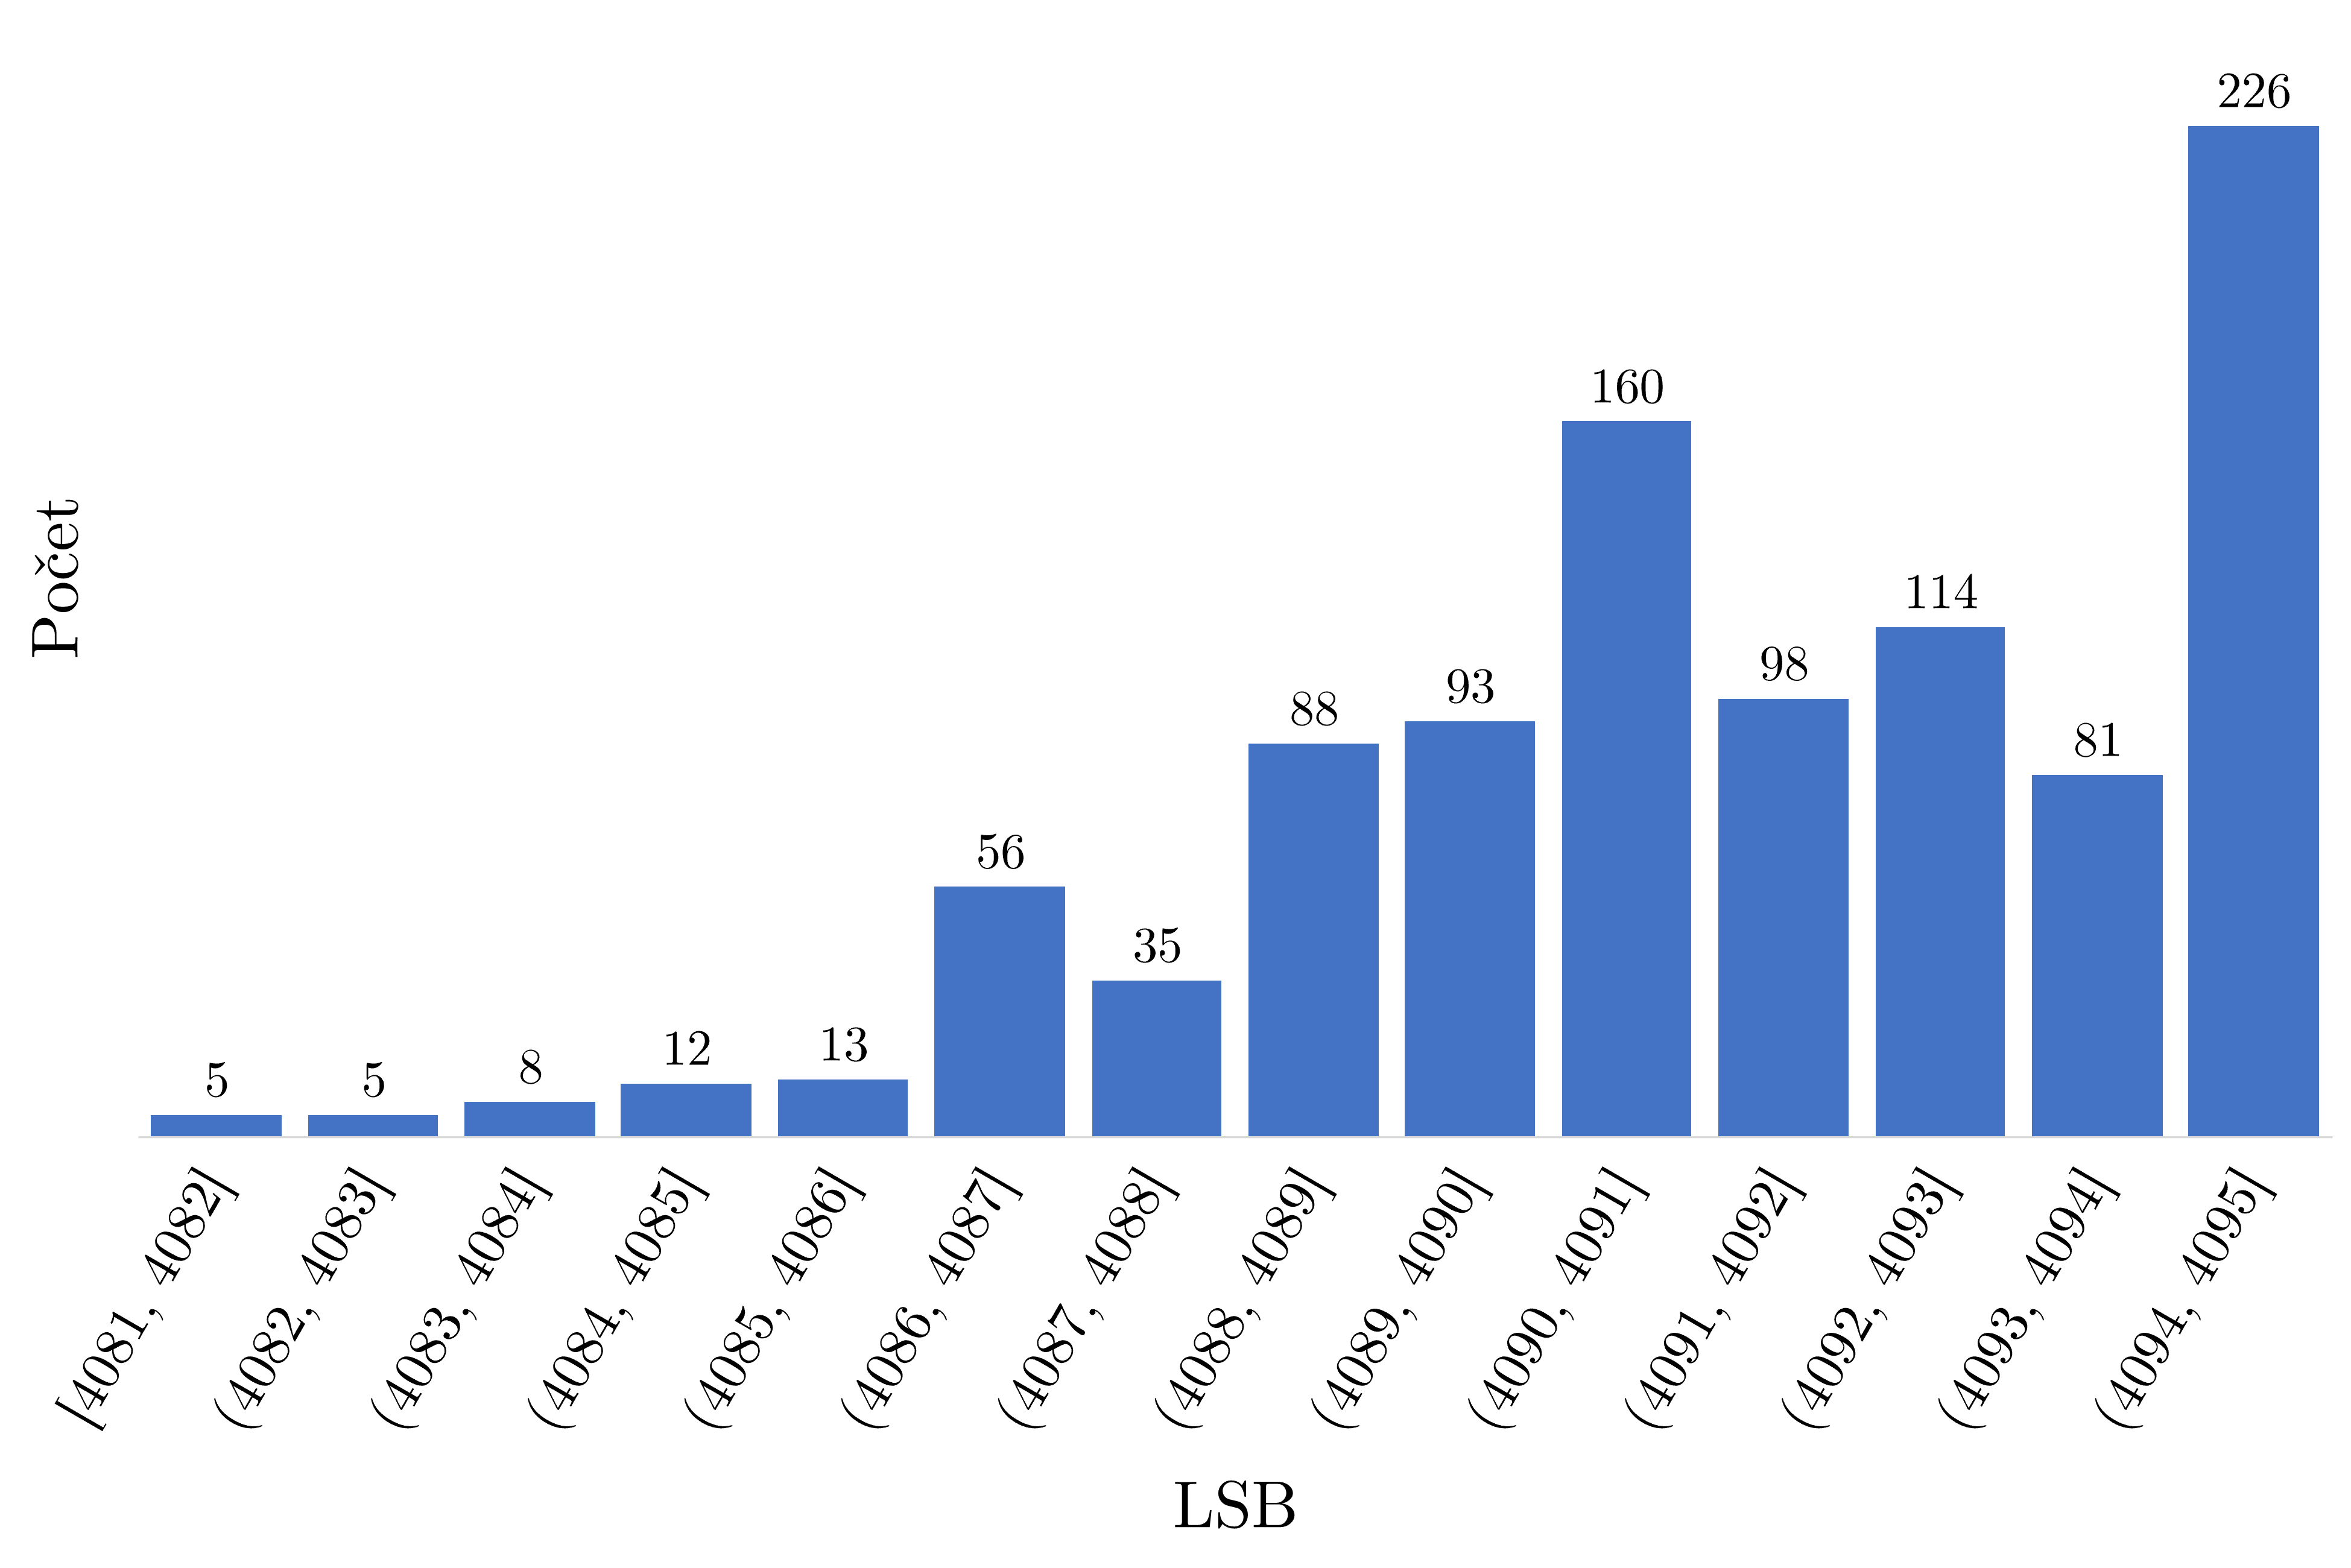
\includegraphics[width=1\textwidth]{graphs/vacuum2_33.png}

\end{figure}
Očekáváné hodnoty pro připojení k $U_{in} = U_{ref} \ V$ jsou $4095$. Střední hodnota naměřených dat je $\mu = 4091.59$ se směrodatnou odchylkou $\sigma = 2.85$. Po převedení naměřených dat na napětí $U_{out} = 3.28 \pm 0.0023 \ V$ je napěťový rozdíl od očekávané hodnoty $U_{in} = U_{ref} = 3.29 \ V$
$U_{offset} = -2.73 \pm 2.29 \ mV$.


\subsection{Charakteristika MCP3561} \label{section:char_mcp}
24bitový AD převodník MCP3561 převádí hodnoty z diferenčního sensoru tlaku. Během měření MCP3561 je zapojeno podle schéma (\ref{fig:mcp3561_connection}) a vnitřní nastavení registrů je následovné $OSR = 256$, $GAIN = 1$, $PRESCALE = 1$, $GAIN = 1$, $BOOST = 1$.
Při této konfiguraci registrů AD převodník má přenosovou rychlost $f_s = 4800 \ kHz$ a efektivní počet bitů $ENOB = 19.5$ bit. Hodnota 1 LSB $= \frac{U_{ref}}{2^{24 - 1}} = 392.07 \ nV$.
\begin{figure}[H]
    \caption{Graf počtu hodnot LSB 24bit AD převodníku MCP3561 při připojení kanálu
        pro diferenční tlakový sensor k referenční zemi.}
    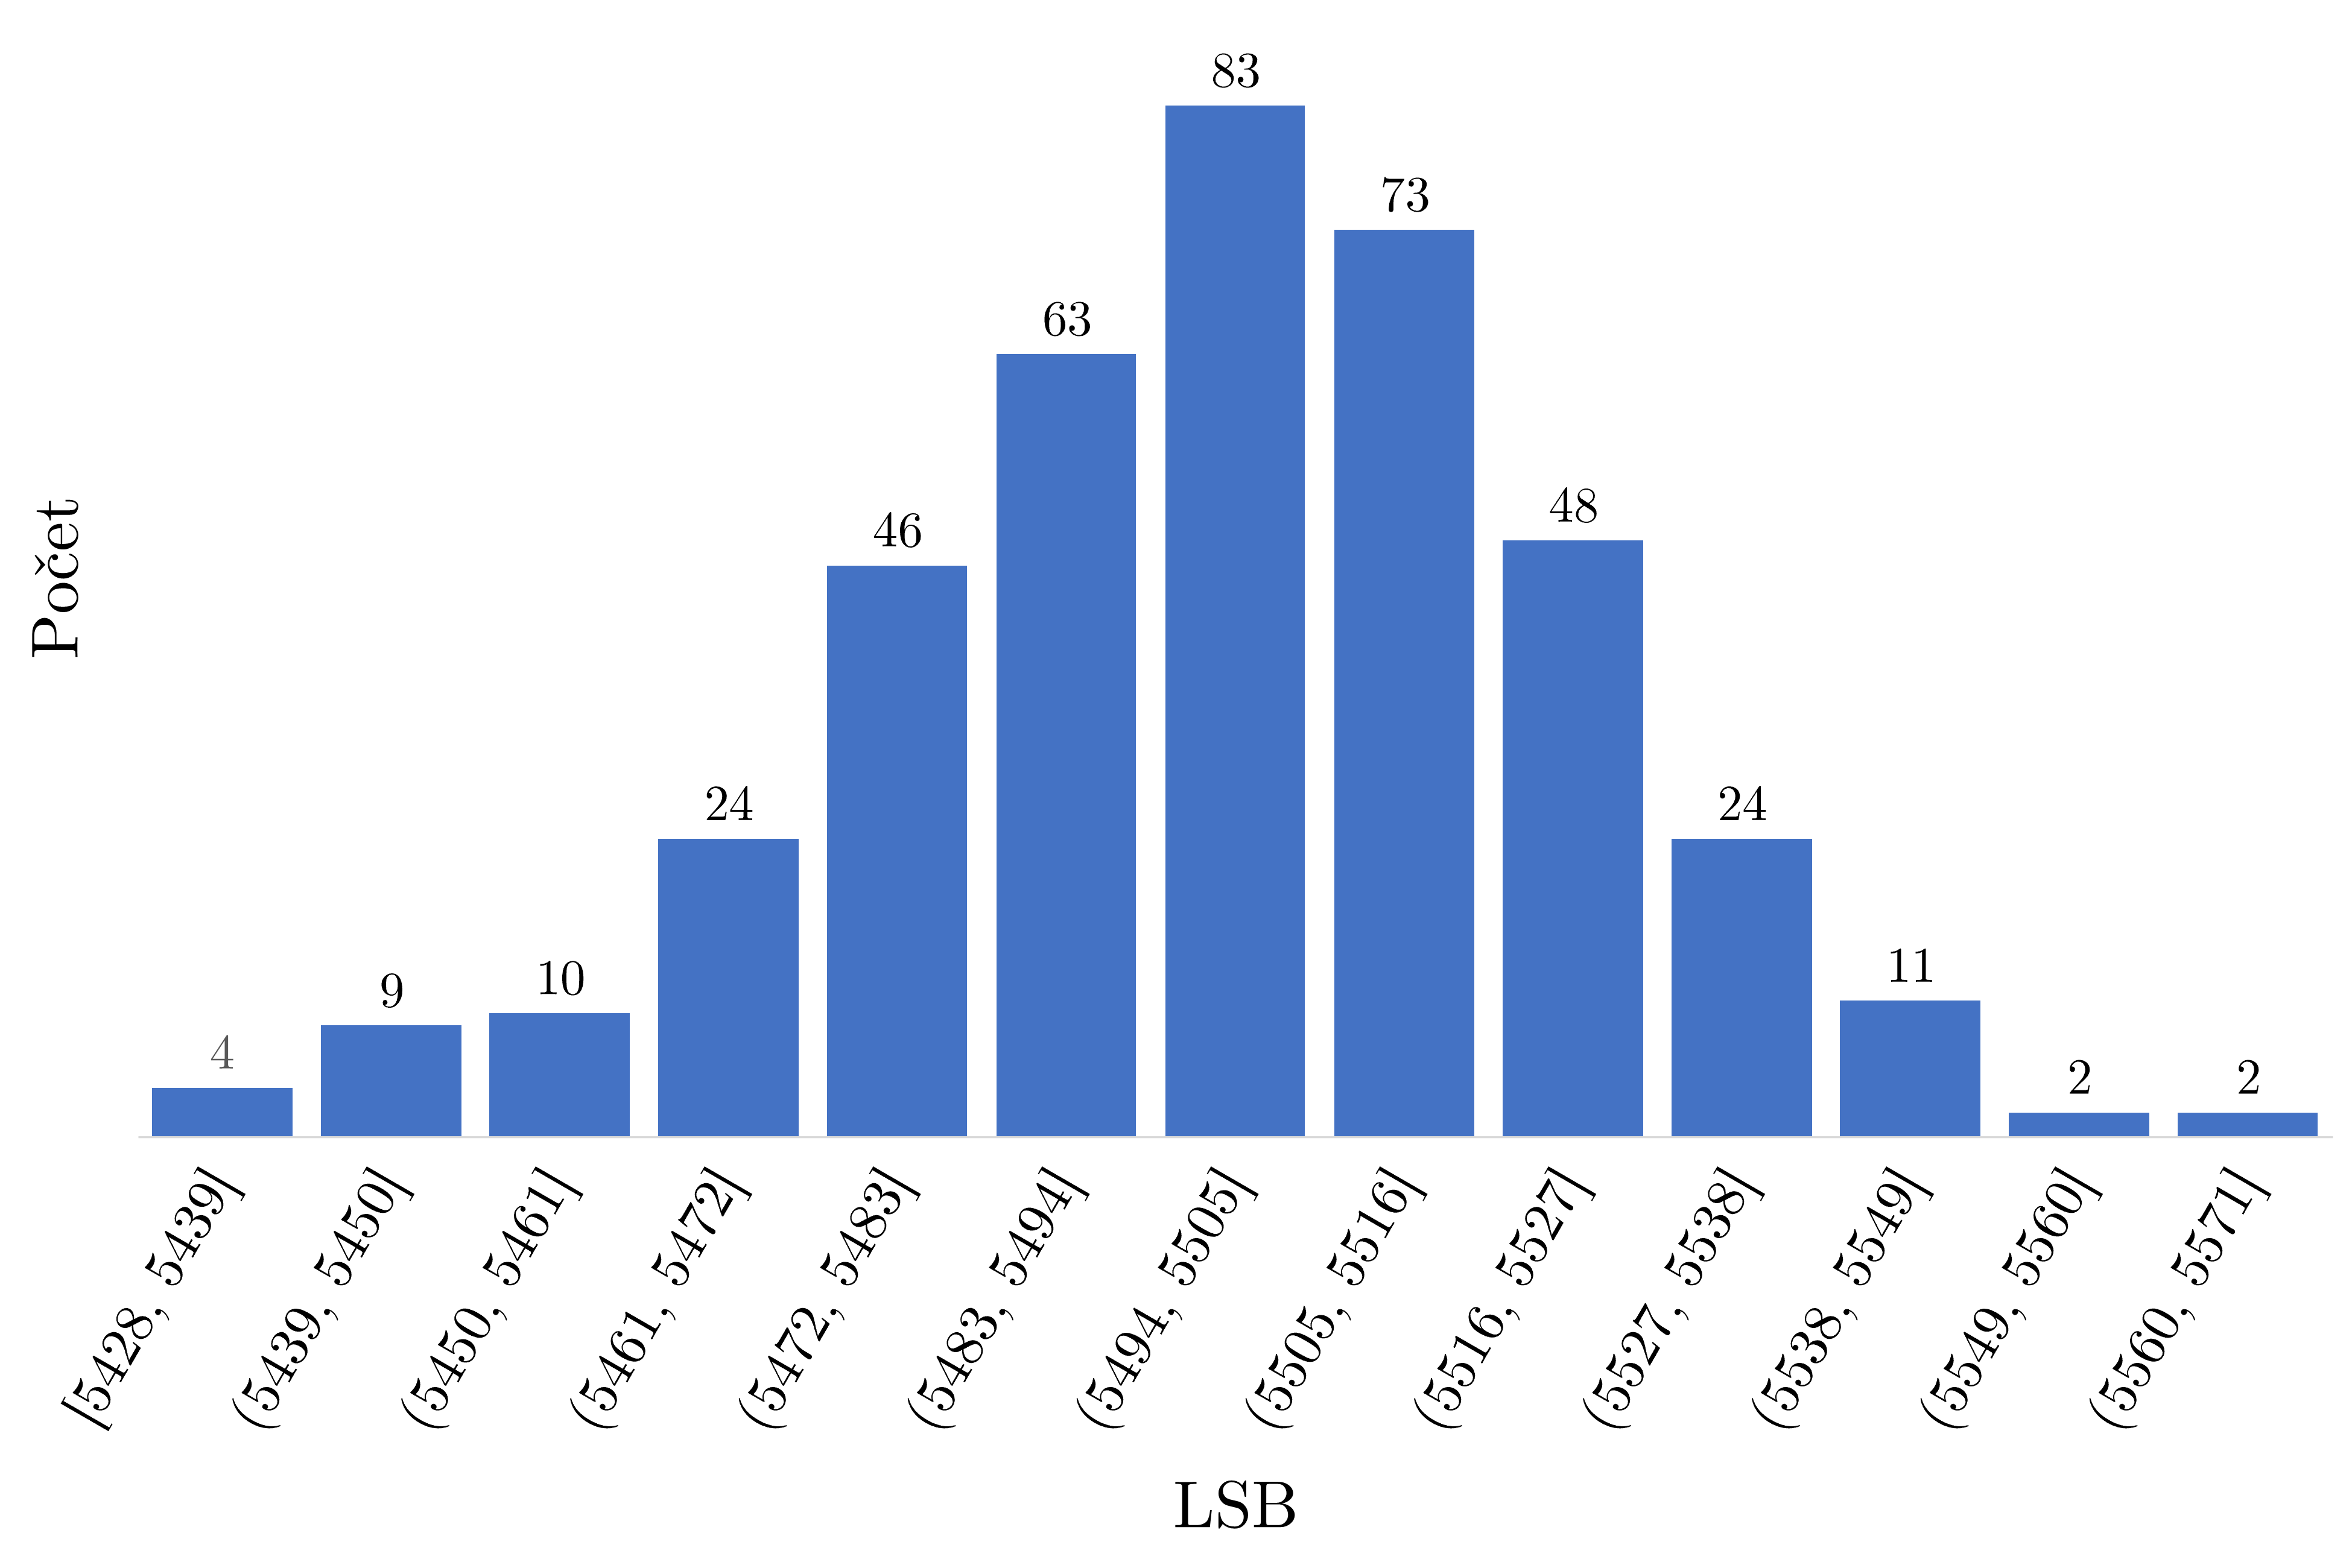
\includegraphics[width=1\textwidth]{graphs/mcp_gnd.png}
\end{figure}
Očekáváné hodnoty pro připojení k referenční zemi je 0. Střední hodnota naměřených dat je $\mu = 5499.17$ se směrodatnou odchylkou $\sigma = 23.09$. Aktuální hodnoty se liší od čekávané o $U_{offset} = 2.15 \pm 0.0090 \ mV$

\begin{figure}[H]
    \caption{Graf počtu hodnot LSB 24bit AD převodníku MCP3561 při připojení kanálu
        pro diferenční tlakový sensor k  $1.63 \ V$.}
    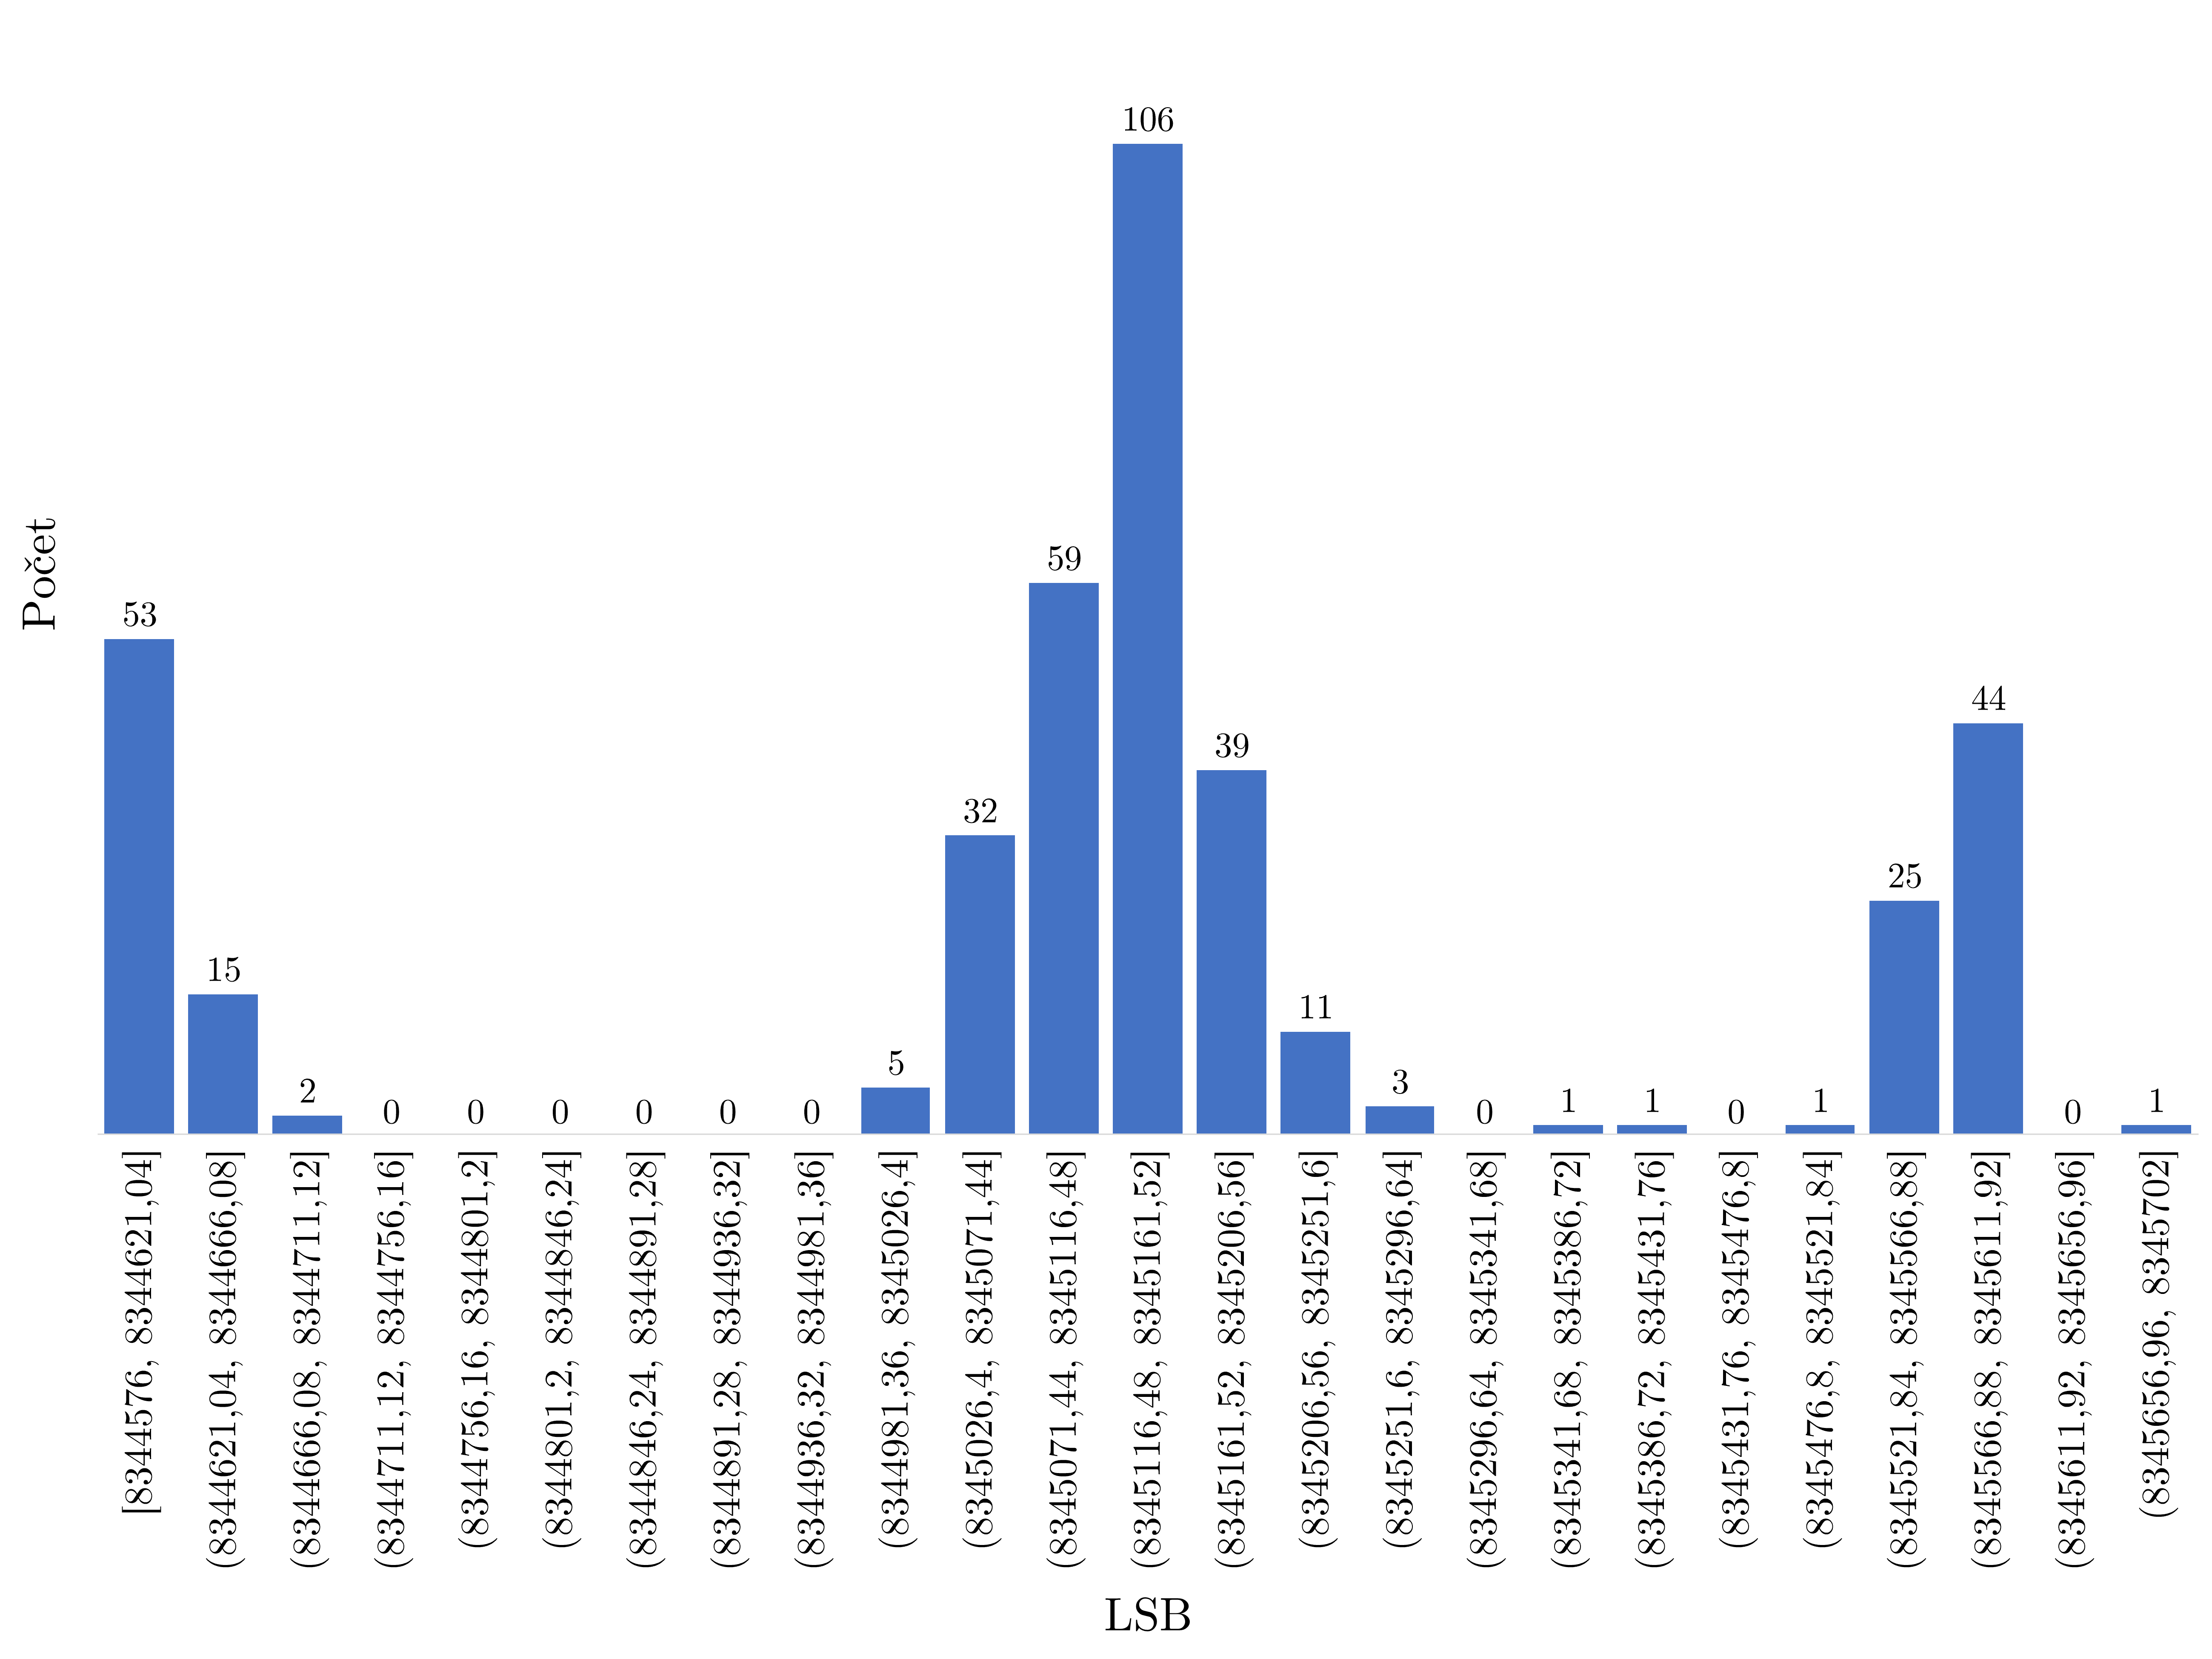
\includegraphics[width=1\textwidth]{graphs/mcp_16.png}
\end{figure}
Očekáváné hodnoty pro připojení k $U_{in} = 1.63 \ V$ jsou $4168728.97$. Střední hodnota naměřených dat je $\mu = 4172558.10$ se směrodatnou odchylkou $\sigma = 145.82$. Po převedení naměřených dat na napětí $U_{out} = 1.63 \pm 0.000057\ V$ je napěťový rozdíl od očekávané hodnoty $U_{in} = 1.63 \ V$
$U_{offset} = 5.99 \pm 0.057 \ mV$.
\par
Po připojení napětí $U_{in} = U_{ref}$ na kanál, AD převodník byl v saturaci a všechny naměřené vzorky byly s hodnotou $U_{ref}$.

\pagebreak
\section{Měření pulzní tlakové vlny}
Pulzní tlaková vlna byla měřena na dobrovolníkovi pomocí navrženého systému CarDi na suprasystolickém tlaku $200 \ mmHg$ a $275 \ mmHg$. Nastavení registrů 24bitového AD převodníku MCP3561 je stejné jako v sekci (\ref{section:char_mcp}).
Postup měření probíhalo podle metody popsané v sekci (\ref{section:metoda_mereni}). Postup tohoto měření je následovný
\begin{enumerate}
    \item Nasazení manžety na levou paži.
    \item Otevření uzavíracího ventilu.
    \item Uzavření regulačních ventilů.
    \item Natlakování pneumatického systému.
    \item Prodleva $20 \ s$ na ustálení tlaku.
    \item Uzavření uzavíracího ventilu.
    \item Prodleva $3 \ s$ na ustálení tlaku.
    \item Měření výstupního signálu diferenčního sensoru tlaku po dobu $3 \ s $.
\end{enumerate}

\pagebreak

\begin{figure}[H]
    % 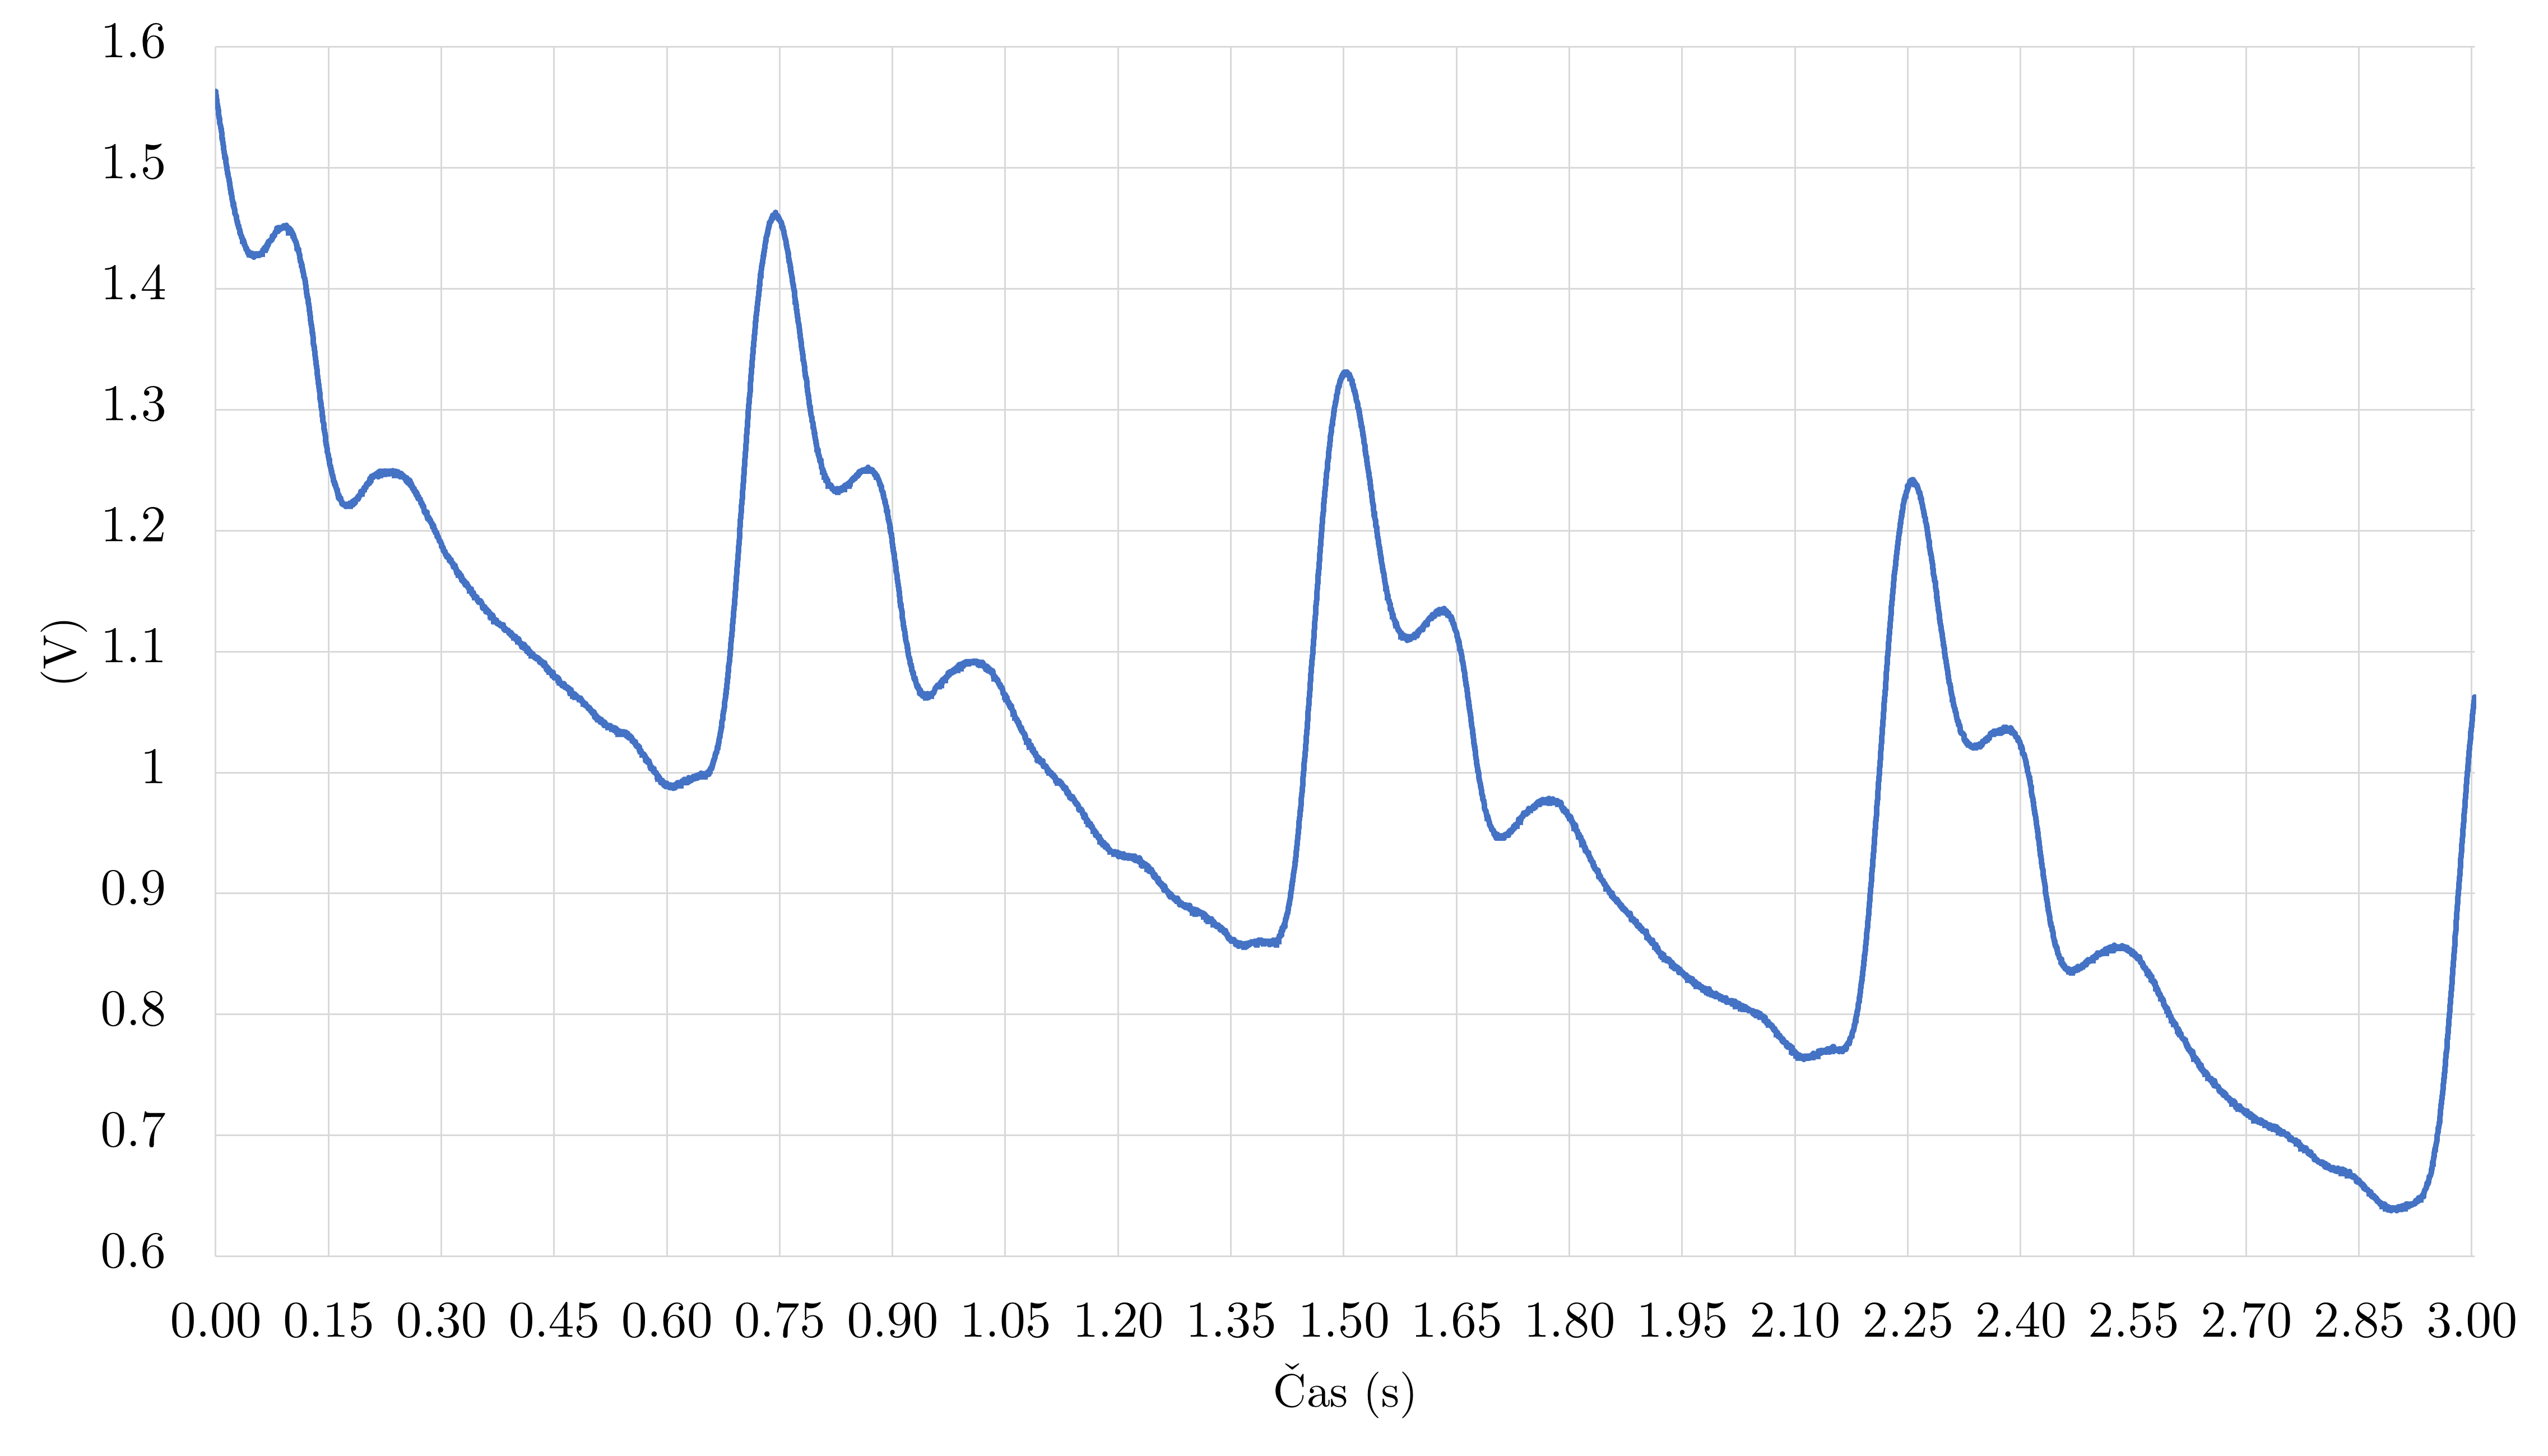
\includegraphics[width=1\textwidth]{graphs/pulzace_fabi_200mmhg.png}
    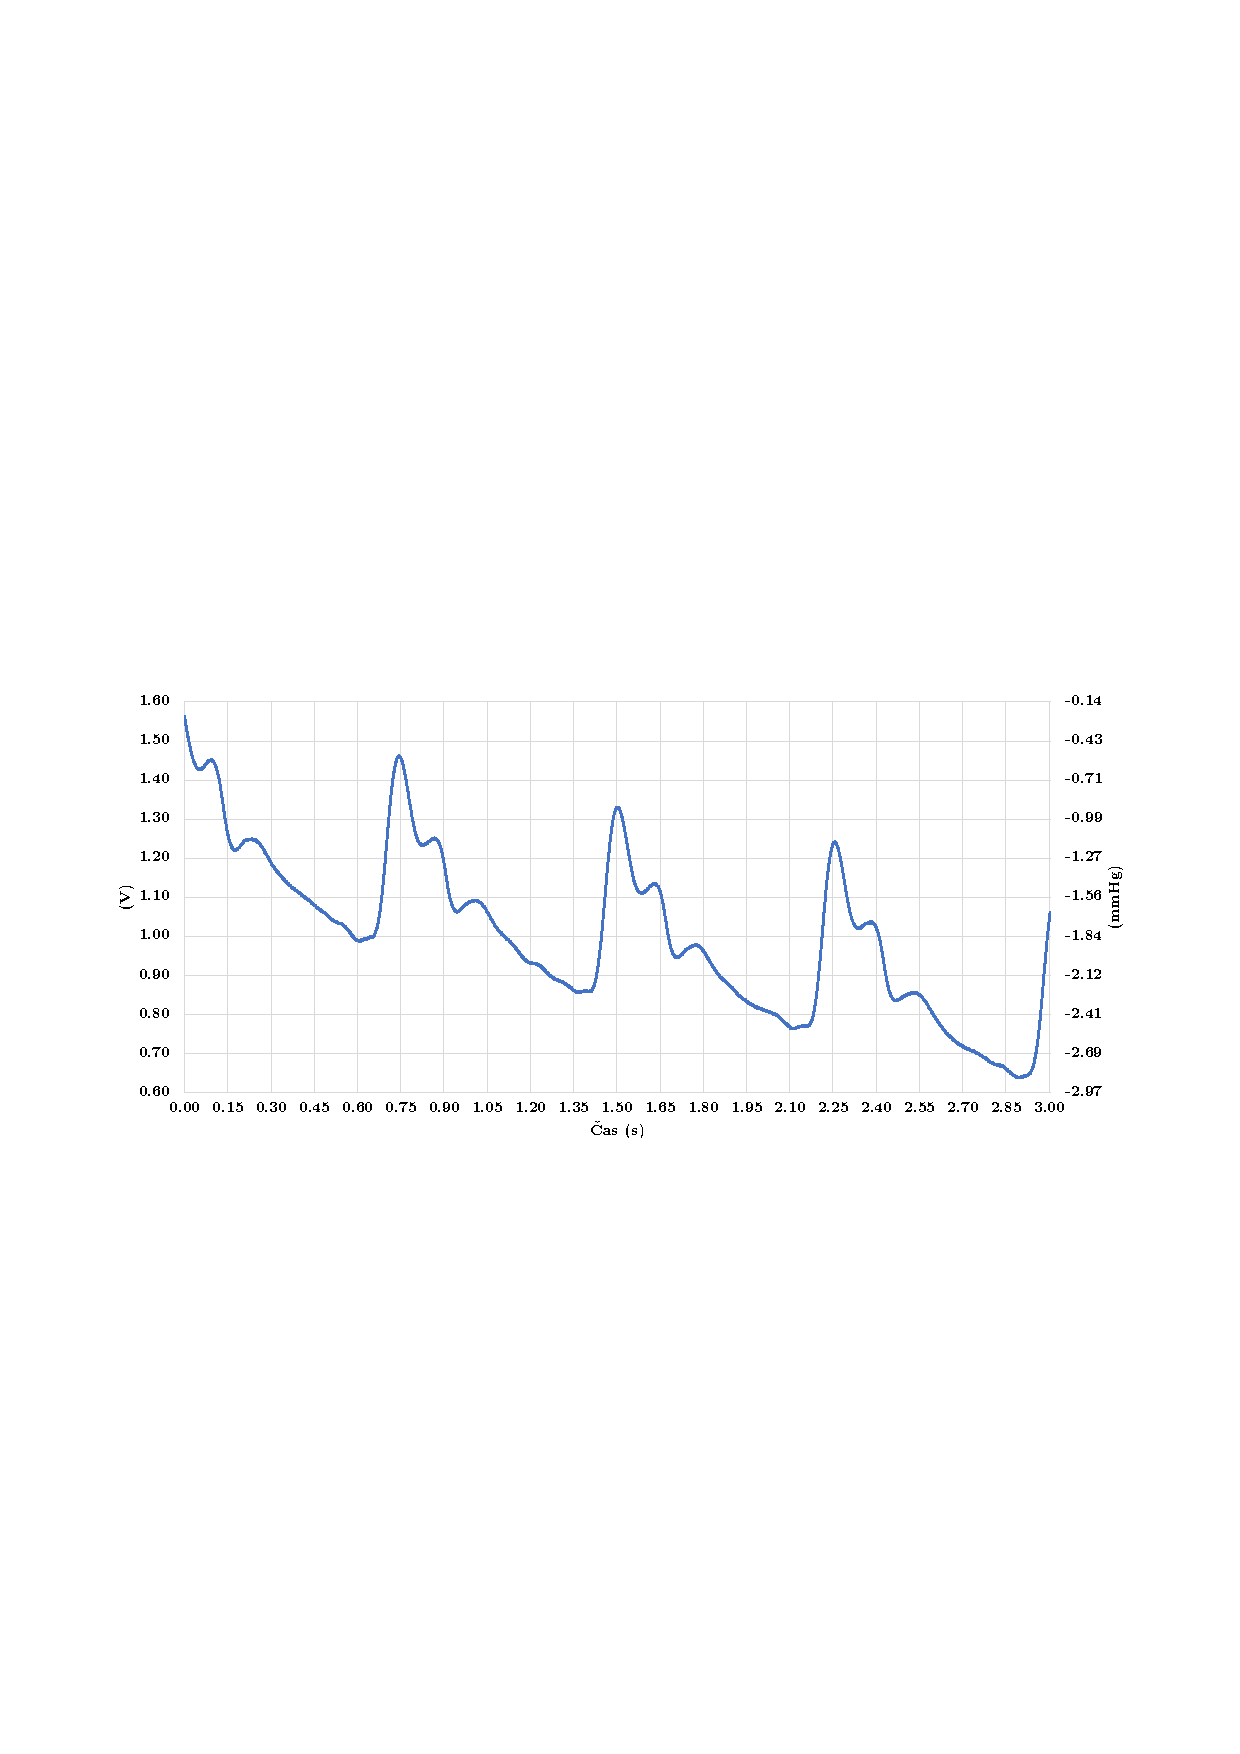
\includegraphics[width=1\textwidth]{graphs/pulzace_fabian_200mmHg.pdf}
    \caption{Pulzní tlaková vlna při manžetním tlaku $200 \ mmHg$}
    \label{fig:pwa_200}
\end{figure}

\begin{figure}[H]
    % 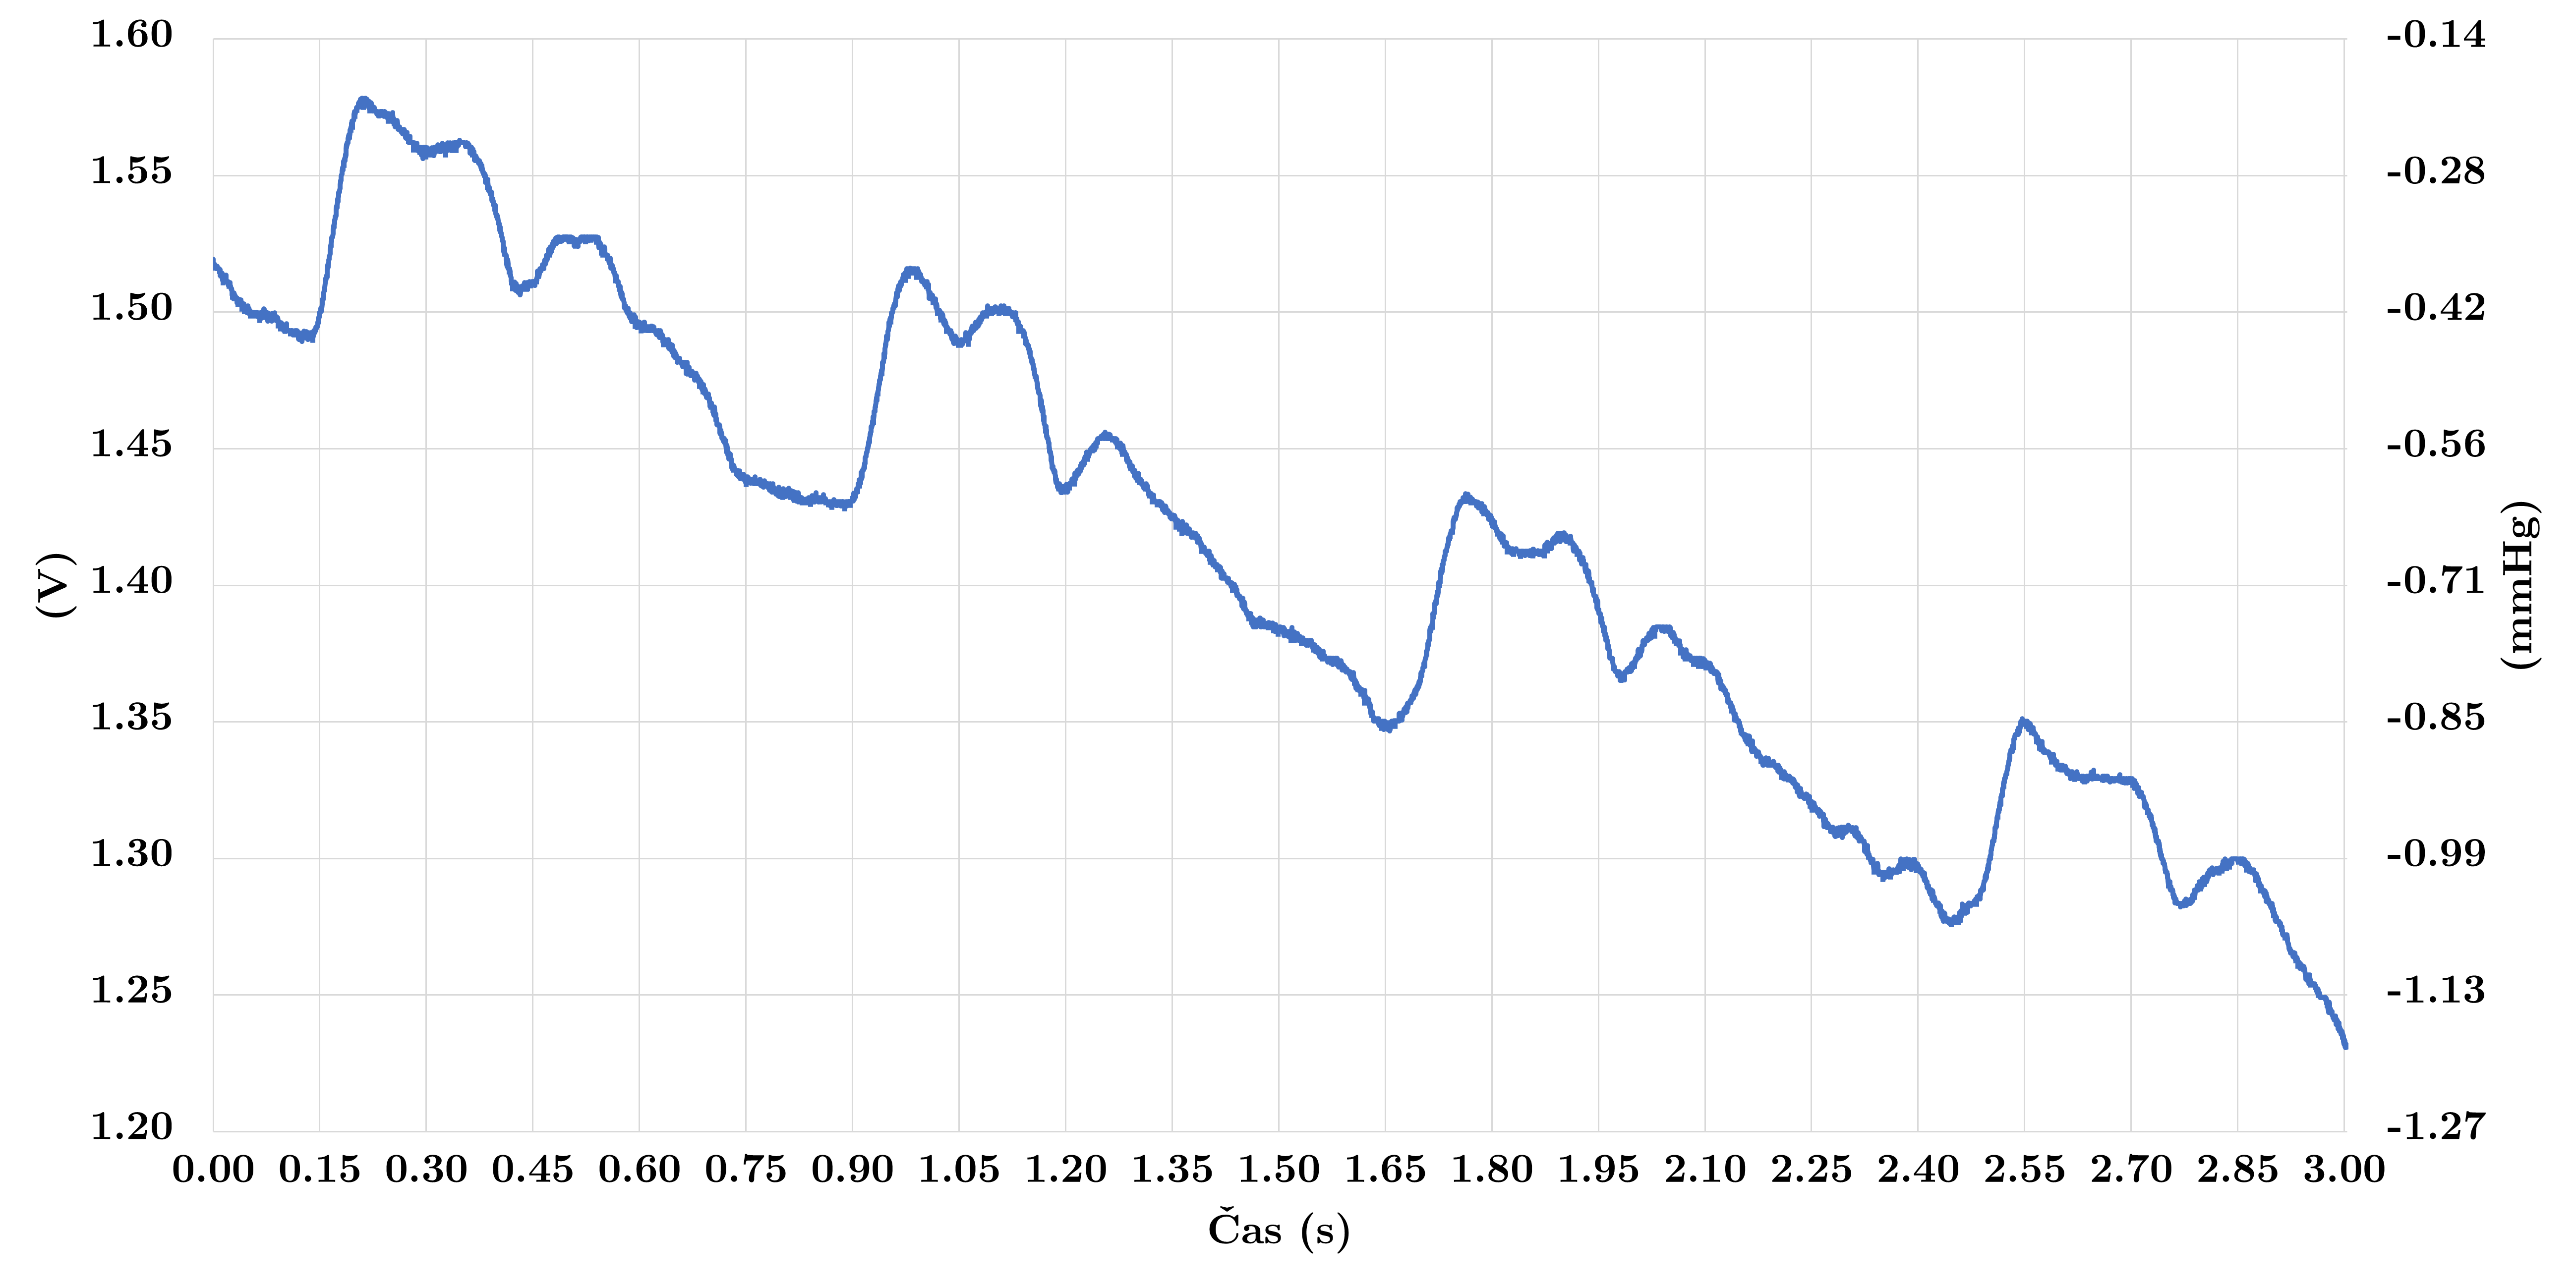
\includegraphics[width=1\textwidth]{graphs/pulzace_fabi_275mmhg.png}
    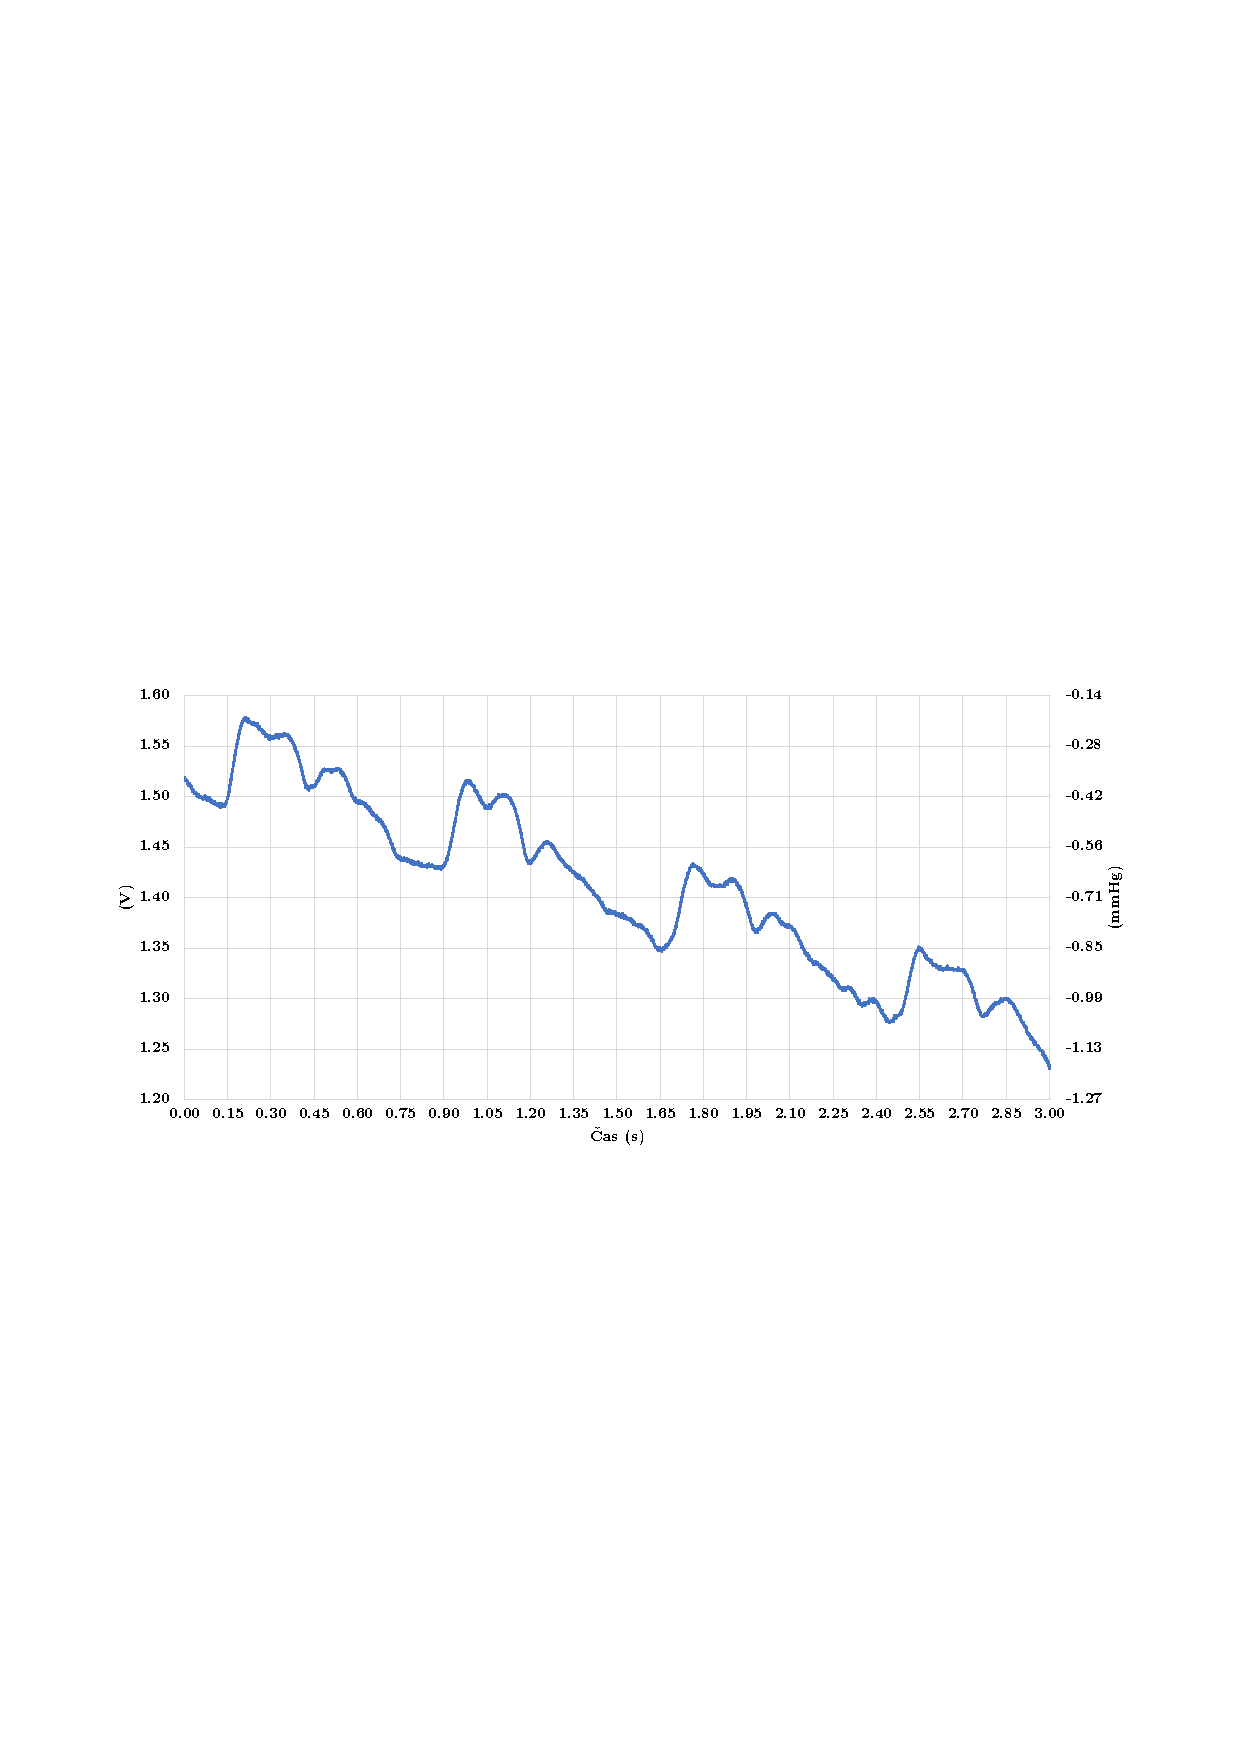
\includegraphics[width=1\textwidth]{graphs/pulzace_fabian_275mmHg.pdf}
    \caption{Pulzní tlaková vlna při manžetním tlaku $275 \ mmHg$}
    \label{fig:pwa_275}
\end{figure}
